%% This is emulateapj reformatting of the AASTEX sample document
%%
\documentclass{emulateapj}
\usepackage{graphicx}
%\usepackage[space]{grffile}
\usepackage{latexsym}
\usepackage{textcomp}
\usepackage{longtable}
\usepackage{multirow,booktabs}
\usepackage{amsfonts,amsmath,amssymb}
\usepackage{url}
\usepackage{hyperref}
\hypersetup{colorlinks=false,pdfborder={0 0 0}}

\newcommand{\vdag}{(v)^\dagger}

\usepackage{natbib}
\renewcommand\floatpagefraction{1.0}
\renewcommand\topfraction{.99}
\renewcommand\bottomfraction{.99}
\renewcommand\textfraction{0.01}
\renewcommand\dbltopfraction{0.99}

\DeclareGraphicsExtensions{.pdf,.png}

\setcounter{totalnumber}{50}
\setcounter{topnumber}{50}
\setcounter{bottomnumber}{50}
\setcounter{dbltopnumber}{50}

\newcommand\fnurl[2]{%
\href{#2}{#1}\footnote{\url{#2}}%
}
\newcommand\A[0]{\mathbf{A}}
\newcommand\B[0]{\mathbf{B}}
\newcommand\C[0]{\mathbf{C}}
\newcommand\I[0]{\mathbf{I}}
\newcommand\F[0]{\mathbf{F}}
\newcommand\G[0]{\mathbf{G}}
\newcommand\GammaMat[0]{\boldsymbol{\Gamma}}
\newcommand\x[0]{\mathbf{x}}

\renewcommand\vec[1]{\mathbf{#1}}
\newcommand\al[0]{\boldsymbol{\alpha}}
\newcommand\asinh[0]{\operatorname{asinh}}

\newcommand\Ghat{{\tilde\GammaMat}}

\newcommand\rhat[0]{\vec{\hat{r}}}
\newcommand\drho{\delta\rho}
\newcommand\mumat{{\boldsymbol{\mu}}}
\newcommand\sF{{\mathcal F}}
\newcommand\Sigcrit{\Sigma_{\rm{cr}}}
\newcommand\zeromat{\mathbf{0}}
\newcommand\Transpose{{\mathrm{T}}}
\newcommand\Dhat{{\tilde D}}

\newcommand\Rein{R_{\rm ein}}
\newcommand\betahat{\hat{\beta}}
\newcommand\tauhat{\hat{\tau}}


\newcommand\crk[1]{\textbf{[CRK: #1]}}  
  
\newcounter{Affiliation}
\newcommand{\aftext}[1]{\refstepcounter{Affiliation}\altaffilmark{\theAffiliation}#1}

\begin{document}


\title{Quantifying Environmental and Line-of-Sight Effects in Models of \\ Strong Gravitational Lens Systems}

%% Use \author, \affil, and the \and command to format
%% author and affiliation information.
%% Note that \email has replaced the old \authoremail command
%% from AASTeX v4.0. You can use \email to mark an email address
%% anywhere in the paper, not just in the front matter.
%% As in the title, use \\ to force line breaks.

\author{Curtis McCully\altaffilmark{\ref{af:LCOGT},\ref{af:UCSB},*} \and 
Charles R. Keeton\altaffilmark{\ref{af:Rutgers}} \and
Kenneth C. Wong\altaffilmark{\ref{af:ASIAA},$\dagger$} \and
Ann I. Zabludoff\altaffilmark{\ref{af:Arizona}}
}

\affil{
\aftext{Las Cumbres Observatory Global Telescope Network, 6740 Cortona Dr Suite 102, Goleta, CA 93117-5575, USA\label{af:LCOGT}}\\
\aftext{Department of Physics, University of California, Santa Barbara, CA 93106-9530, USA\label{af:UCSB}}\\
\aftext{Department of Physics and Astronomy, Rutgers, the State University of New Jersey, 136 Frelinghuysen Road, Piscataway, NJ 08854, USA.\label{af:Rutgers}}\\
\aftext{Institute of Astronomy and Astrophysics, Academia Sinica (ASIAA), P.O. Box 23-141, Taipei 10617, Taiwan
\label{af:ASIAA}}\\
\aftext{Steward Observatory, University of Arizona, 933 North Cherry Avenue, Tucson, AZ 85721\label{af:Arizona}}
}
\altaffiltext{*}{\email{}{cmccully@lcogt.net}}
\altaffiltext{$\dagger$}{EACOA Fellow}


\begin{abstract}
Matter near a gravitational lens galaxy or projected along the line of sight (LOS) can affect strong lensing observables by more than contemporary measurement errors. We simulate lenses with realistic three-dimensional mass configurations (including voids), and then use lens models to quantify biases and uncertainties associated with three different ways of treating the environment and LOS.  (1) Ignoring mass outside the lens yields poor fits and biased results.  (2) Adding an external shear in the lens plane can account for tidal stretching from galaxies at the lens redshift or in the background, but it requires corrections for external convergence and cannot fully reproduce the more complicated effects from galaxies in the foreground.  (3) Our new framework for 3-D lensing includes convergence self-consistently and recovers lens model parameters without bias and with scatter limited mainly by the lens profile degeneracy.  We identify the physical combination of mass, projected distance from the lens, and offset from the lens redshift that determines whether a perturbing galaxy needs to be treated exactly or can be treated with the 3-D tidal approximation.  We show that foreground structures have a stronger effect on the lens potential than background structures.  There is dramatic variation in the net strength of environment/LOS effects across different lens fields; modeling fields individually yields stronger priors on $H_0$ than ray-tracing through N-body simulations.  Asymmetric lens systems produced by highly elliptical lens galaxies are less sensitive to the lens profile degeneracy, so they offer appealing targets for precision lensing.
\end{abstract}

%\keywords{globular clusters: general --- globular clusters: individual(\objectname{NGC 6397},
%\object{NGC 6624}, \objectname[M 15]{NGC 7078},
%\object[Cl 1938-341]{Terzan 8})}
\maketitle


%%%%%%%%%%%%%%%%%%%%%%%%%%%%%%%%%%%%%%%%
\section{Introduction}
%%%%%%%%%%%%%%%%%%%%%%%%%%%%%%%%%%%%%%%%
% Reset the footnote counter because star and dagger count as footnotes
\setcounter{footnote}{0}
%%%%%%%%%%%%%%%%%%%%%%%%
Strong gravitational lensing is an important probe for many facets of cosmology. Analysis of strong lenses has led to constraints on the masses and properties of dark matter halos of galaxies \citep[e.g.,][]{Keeton98,Treu06,Koopmans06,Barnabe09,Auger10,Treu10,Lagattuta12,Hezaveh15}, substructure in galaxy halos \citep[e.g.,][]{Mao98,Metcalf01,Dalal02,Vegetti14,Hezaveh14}, and the Hubble constant, independent of the cosmic distance ladder \citep[e.g.][]{Refsdal64,Keeton97_PG1115,Kochanek03,Saha06,Oguri07,Suyu10,Suyu13}. Strong lensing may also be employed to constrain the properties of dark energy \citep[e.g.,][]{Turner90,Linder04,Linder11,Cao12,Treu13}.

In recent years, both the quantity and quality of strong lens data have improved. There are now roughly a hundred known lensed quasars (e.g.,\ \fnurl{CASTLeS}{http://www.cfa.harvard.edu/castles/}; \citealt{SQLS,CLASS}) and a comparable number of strongly lensed galaxies \citep[e.g.,][]{Bolton08,Cassowary}. These samples will increase dramatically in the near future with LSST \citep[e.g.,][]{LSST, Coe09, Oguri10, Collett15}. Here, we focus on quasar lenses because the compact source can vary rapidly enough to enable measurements of lens time delays (though much of this discussion also applies to strongly lensed supernovae; \citealt{Kelly15}). The relative positions and fluxes of quasar images are routinely measured to high precision using the \textit{Hubble Space Telescope} \citep[e.g,.][and references therein; CASTLeS Collaboration]{Lehar00,Sluse12}. Our understanding of gravitational lenses and the constraints they place on cosmology is no longer limited by observations, but by systematic uncertainties. 

One of the key issues is that lens galaxies are not isolated systems. Matter in the environment of the lens galaxy and projected along the line of sight (hereafter ENV/LOS) can produce perturbations in the lensing potential that cannot be ignored as we enter the era of ``Precision Lensing'' (typically defined by the goal of constraining the Hubble constant to $1\%$). To lowest order, using the ``tidal approximation,'' perturbing galaxies contribute ``external convergence,'' which produces extra (de-)magnification, and ``external shear,'' which stretches the images of the source, transforming circles to ellipses. External convergence is one of the dominant components of the uncertainty budget for measurements of the Hubble constant \citep{Suyu12}. Our goal for this work is to quantify the effects of mass outside the main lens galaxy on the measured cosmology,\footnote{Here we focus on the Hubble constant, but similar arguments apply for time-delay cosmography measurements that have been proposed to be used to measure dark energy \citep{Treu13}.} using three different methodologies for treating the lensing ENV/LOS.

The first method (which we term ``Lens-Only'') neglects mass outside the main lens altogether.  This approach is almost surely produces biased constraints on the Hubble constant, and so it is rarely used in studies that derive constraints on precision cosmology, but it still appears in some studies that focus on lens and source properties \citep[e.g.][]{Calanog14, Hezaveh13}.

The second method (``Lens+Shear'') accounts for tidal effects in the lens plane by treating the magnitude and direction of the external shear as free parameters to be optimized for individual lens systems. This widely-used approach has several limitations. First, the tidal approximation neglects higher-order effects beyond shear, which may be significant for objects sufficiently close to the optical axis. This approach also neglects non-linear effects that arise from having mass in multiple redshift planes \citep[][]{McCully14,Jaroszynski12}. Also, lens models cannot directly constrain the external convergence because of the mass sheet degeneracy \citep{Falco85}.  To avoid biases in the derived cosmological parameters, corrections for external convergence must be applied using additional constraints such as weak lensing \citep{Nakajima09, Fadely10} or the number density of galaxies near the lens \citep{Suyu10, Suyu13, Collett13} calibrated by ray tracing through cosmological simulations \citep[e.g.,][]{Hilbert09}. \citet{Schneider13} have raised concerns because these corrections are calibrated on scales much larger than those relevant for strong lensing.  Also, they are derived from statistical studies that may have limited applicability to individual lens environments. Finally, the shear derived from lens models does not always match the shear calculated from modeling the ENV/LOS directly \citep{Wong11}.

The third method (``3-D Lens'') is to build full, three-dimensional mass models that explicitly account for mass in the environment and along the LOS.  We now have extensive photometric and spectroscopic data for $\sim25$ strong lensing systems \citep{Momcheva06,Williams08,Momcheva15}, which we can use to assign mass throughout a ``beam'' that is centered on the lens and runs from the observer to the source \citep[see][]{Wong11}.  While our approach is more complicated and observationally expensive, our models have a direct connection between the convergence and shear in lens models and the physical mass in the beam. The multi-plane lensing framework we developed in \citet{McCully14} (hereafter M14) allows us to balance accuracy and efficiency when computing lensing effects with 3-D mass models.

One goal for this paper is to compare lens parameters recovered from the three types of models (Lens-Only, Lens+Shear, and 3-D Lens) to identify biases and uncertainties that may be present in the methodologies.  A second goal is to address three questions about ENV/LOS effects:
Which perturbing galaxies are the most important?
What is the range of ENV/LOS contributions?
Which image configurations produce the strongest constraints on the Hubble constant?
In Section \ref{sec:3DMassModels} we describe how our 3-D mass models are constructed and review the multi-plane lensing formalism derived in M14, adding the capability to include voids in the lens models (Section \ref{sec:Voids}).  In Section \ref{sec:Individual} we discuss which individual galaxies produce the largest ENV/LOS effects. We then examine the recovered parameters from realistic 3-D mass models and compare to fits with only an external shear in Section \ref{sec:los_vs_shear}. Based on these results, we compare the ENV/LOS effects for different lens fields in Section \ref{sec:Environments}. We finish by showing that certain lensed image configurations produce stronger constraints on the Hubble constant in Section \ref{sec:ImageConfigs}.  Throughout this paper we assume a cosmology with $\Omega_M = 0.274$, $\Omega_\Lambda = 0.726$, and $H_0 = 71$ km s$^{-1}$ Mpc$^{-1}$.

%%%%%%%%%%%%%%%%%%%%%%%%%%%%%%%%%%%%%%%%
\section{Gravitational Lensing Using 3-D Mass Models}
\label{sec:3DMassModels}
%%%%%%%%%%%%%%%%%%%%%%%%%%%%%%%%%%%%%%%%

\subsection{Building 3-D Mass Models from Observations}

The first step in building 3-D lens models is to convert photometric and spectroscopic data into mass models. We construct our models using an updated version of the methodology in \citet{Wong11}, which we briefly summarize here. We start by assigning redshifts to the LOS galaxies that lack spectroscopy. If the field is in the SDSS footprint, we assign photometric redshifts from \crk{REF}. If not, we draw from a smoothed version of the spectroscopic redshift distribution in that particular field. We model galaxies as singular isothermal spheres with velocity dispersions and truncation radii drawn from scaling relations (including scatter) derived from a galaxy-galaxy weak lensing analysis in the CFHTLS \citep{Brimioulle13}. For lenses that lie in a group or cluster, we treat the group member galaxies in a slightly different way. We compute a total dynamical mass for the group (\citealt{Girardi98,Momcheva06,Momcheva15}; Wilson et al.\ in preparation) and apportion the mass between the group dark matter halo and the group galaxies. The dark matter halo is assumed to be a spherical NFW profile. The halo concentration is taken from the mass-concentration relation from simulations by \citet{Zhao09}, with an assumed scatter of 0.14 dex \citep{Bullock01}. The fraction of the total group mass assigned to the halo, $f_{\rm{halo}}$, is randomly drawn from a uniform distribution such that the group galaxies are not truncated below twice their effective radii, nor beyond their $R_{200}$ (the radius at which the mean density enclosed is 200 times the matter density at that redshift). The remainder of the mass, $(1-f_{\rm{halo}})M_{\rm{group}}$, is assigned to the group galaxies, which are scaled such that they have the same density at their truncation radii. All group galaxies and the group halo are assumed to be in the same redshift plane as the lens, even though there may be slight redshift differences due to peculiar velocities. For this study, we fix the ENV/LOS mass model. We will consider the uncertainties in generating these mass models in a forthcoming work (Wong et al.\ in preparation). 

\subsection{Multi-plane Lensing}

In our previous paper (M14; see \citealt{Schneider14} for an alternative derivation.), we presented a hybrid framework for multi-plane gravitational lensing that fills the gap between using the full multi-plane lens equation (which can be computationally expensive) and treating everything as a simple external shear (which omits higher-order effects that can be significant for objects projected near the lens). The framework can handle any mixture of ``main'' planes (strong lenses) that are given full treatment and ``tidal'' planes (weak lenses) that are treated using the tidal approximation. Even when it uses the tidal approximation, our framework includes non-linear effects associated with having mass at different redshifts.  (Sections \ref{sec:Individual} and \ref{sec:los_vs_shear} discuss the objective criterion we use to determine which perturbers can be treated with the tidal approximation.)

Our framework can be used to calculate all of the standard lensing observables. The general expressions for the lens equation, magnification tensor, and time delay are as follows:
\begin{eqnarray}
\x_{j} &=& \B_i \x_1 - \sum_{\ell \in \{\ell_\mu<j\}} \C_{\ell j} \al_\ell(\x_\ell), \label{eqn:lenseqn}\\
\A_{j} &=& \B_i - \sum_{\ell \in \{\ell_\mu<j\}} \C_{\ell j} \GammaMat_\ell \A_\ell, \\
T &=& \frac{1}{2} \x_s \cdot \F_s \x \nonumber \\
&&+ \sum\limits_{\ell \in \{\ell_\mu\}}\left[\frac{1}{2}\tau_{\ell s} \x_\ell \cdot \al_\ell -\frac{1}{2}\x_s \cdot \G_{\ell s}\al_\ell -\tau_{\ell s}\phi_\ell \right],
\end{eqnarray}
where the sums run over main lens planes (i.e., those that are not treated with the tidal approximation), $\al_\ell$ is the deflection in main plane $\ell$, and  
\begin{equation}
\tau_{i\,j} = \frac{ 1 + z_i}{c} \frac{D_i D_j}{D_{i\,j}}.
\end{equation}
Note that each main plane needs to be evaluated using the positions $\x_\ell$, which are not generally the same as the positions $\x_1$ on the sky and must be computed with the lens equation. This distinction gives rise to non-linearities that cannot be mimicked by a simple shear. Our framework is therefore more accurate than fitting a simple shear, but it is also more efficient than the full multi-plane lens equation because the recursive sums include only main planes.  All of the tidal effects are characterized by the following matrices:
\begin{eqnarray}
\B_j &=& \I - \sum\limits_{i=1,i\not \in \{\ell_\mu\}}^{j-1}\beta_{ij}\GammaMat_i \B_i, \\
\C_{\ell j} &=& \beta_{\ell j} \I - \sum\limits_{i=\ell+1, i\not\in\{\ell_\mu\}}^{j-1} \beta_{\ell i}\GammaMat_i\_{\ell i}, \label{eqn:cmatdef}\\
\F_j &\equiv& 
%\tau_{j-1} \B_{j}-\tau_{j-1} \B_{j-1} \ =\ 
  - \sum\limits_{i=1,i\not \in \{\ell_\mu\}}^{j-1} \tau_{is}\GammaMat_i\B_i, \\
\G_{\ell j}&\equiv& 
%\tau_{j-1} \C_{\ell j}-\tau_{j-1} \C_{\ell \,j-1} \nonumber \\
% &=&\ 
 \tau_{\ell s}\I- \sum\limits_{i=\ell+1,i \not \in \{\ell_\mu\}}^{j-1} \tau_{is}\GammaMat_i\C_{\ell i}
\end{eqnarray}
where 
\begin{equation}
\beta_{i\,j} = \frac{D_{i\,j} D_s}{D_{j}D_{i\,s}}.
\end{equation}
These matrices can be computed once at the start of any lens modeling analysis and stored for repeated use.

Note that if we take the observer to be in plane $i =0$, we can write $\beta_{0\,j} = 1$ and $\tau_{0\,j} = 0$. We then realize that the $\B$ and $\C$ matrices are related, as are the $\F$ and $\G$ matrices:
\begin{equation}\label{eqn:BC-FG}
\B_j = \C_{0 \, j}
\qquad\mbox{and}\qquad
\F_{j} = \G_{0 \, j}.
\end{equation}

If there is a single main plane, the multi-plane lens equation reduces to
\begin{equation}
\x_s = \B_s \x_1 - \C_{\ell s} \al(\B_\ell \x_1).
\end{equation}
This resembles the standard single-plane lens equation except that $\B_\ell$ appears in the argument of the deflection of the main lens galaxy, leading to non-linear effects that we quantify and explore using our numerical results in the following sections.

\subsection{Setting the Smooth Background Density}
\label{sec:Voids}

In traditional single-plane lensing, it is reasonable to assume that the lens galaxy does not significantly contribute to the overall geometry of the universe, and thus to place it on top of a smooth background density given by the mean density of the universe.  As we begin to include more and more galaxies along the line sight, however, the cosmological effects become non-negligible.  Simply adding the galaxies on top of the mean density would lead to biased results.  If our mass models were 100\% complete, there should be no smooth background component at all.  In practice, we need to find an intermediate approach that scales the background density to account for incompleteness in our mass models (which can arise, for example, from having flux-limited photometric and spectroscopic data).

There are several ways we could do this.  One possibility is to start with an \emph{empty} beam and add both galaxies and a smooth density field.  However, we would still need to account for the mean density of the universe outside the beam when computing cosmic distances.  A different approach, which we prefer, is to start with a \emph{filled} beam and subtract a smooth density field that corresponds to the completeness of our mass model.  Then we can compute cosmic distances using the standard filled beam expressions but still account for the lensing effects produced by having a smooth background density that is less than the mean density.  In our framework, we can achieve the subtraction by inserting redshift planes with negative mass density in between the planes that contain galaxies.  In the limit of a large number of thin planes, the sums over ``void'' planes becomes integrals that we now derive.

Consider a plane that represents the projection of a thin slab extending from proper distance $r_p$ to $r_p+dr_p$.  If the density contrast within this slab is $\drho_p = \rho_p - \bar\rho_p$, the lensing effects are characterized by a convergence
\begin{equation}
  d\kappa = \frac{\drho_p\,dr_p}{\Sigcrit}
\end{equation}
where the critical surface density for lensing is
\begin{equation}
  \Sigcrit = \frac{c^2}{4 \pi G} \frac{D_s}{D_\ell D_{\ell s}}
\end{equation}
Converting to comoving distances $X(z)$, we can write
\begin{equation}\label{eqn:dkappa}
  d\kappa = \frac{4 \pi G}{c^2}\frac{X (X_s - X)}{X_s} \frac{\drho_p}{(1+z)^2} dX.
\end{equation}
In order to achieve the desired subtraction, we set the density contrast to be
\begin{equation}
  \drho_p = -f(z) \bar{\rho}(z) 
\end{equation}
where $f(z)$ is the mass completeness in our models (which can vary with redshift; see Section \ref{sec:setup}), and the mean density of the universe at redshift $z$ is $\bar{\rho}(z) = \rho_{c} \Omega_m (1 + z)^3$, where $\rho_{c} = 3 H_0^2 / 8 \pi G$ is the critical density of the universe today.

We now need to incorporate the ``void'' planes into our LOS framework.  The general expression for the $\C$ matrix\footnote{The following argument also applies to the $\B$ matrices since they are a subset of the $\C$ matrices (see eq.\ \ref{eqn:BC-FG}).} between redshifts $z_i$ and $z_j$ is given in equation \ref{eqn:cmatdef}. The sum in that equation now includes both tidal and void planes, but we can handle the sums over void planes by redefining the $\beta$ factors as follows.  If there is only mean density between redshifts $z_i$ and $z_j$, then there are no planes in the sum and hence $\C_{i j} = \beta_{i j } \I$: the connection between the planes is an isotropic tensor that depends on distance ratios. Now suppose there are only void planes between $z_i$ and $z_j$, with $\GammaMat_k \rightarrow \Delta \kappa_k \I$. Since void planes are isotropic, $\C_{i j}$ will still be isotropic. Therefore, let us define a new $\betahat_{i j}$ such that $\C_{i j} = \betahat_{i j} \I$. We point out that $\C_{i k } = \betahat_{i k} \I$ for all $i < k < j$. Using this definition along with the definition of $\C$ in equation \ref{eqn:cmatdef}, we see that $\betahat_{i j}$ must follow the recursion relation
\begin{equation}
\label{eqn:betahatdef}
\betahat_{i j}  = \beta_{i j} - \sum \limits_{k = i +1}^{j -1} \betahat_{i k} \beta_{k j} \Delta \kappa_k.
\end{equation}
Now if plane $j$ is a tidal plane that includes a galaxy, we write the shear tensor as $\GammaMat_j + \Delta \kappa_j \I$. Then,
\begin{equation}
\C_{i \, j +1} = \betahat_{i j}  - \betahat_{j \, j+1} \GammaMat_j \C_{i j},
\end{equation}
where we have used $\beta_{k \, k+1} = \betahat_{k\, k+1}$.

Next we consider $j +1$ as a void plane and $j + 2$ as a tidal plane and find that
\begin{eqnarray}
\hspace*{-0.45cm}\C_{i \, j+2} &=& \betahat_{i \, j+2} - \betahat_{j \, j + 2} \GammaMat_j \C_{i j}\\
\hspace*{-0.45cm}\C_{i \, j+3} &=& \betahat_{i \, j+3} - \betahat_{j \, j + 3} \GammaMat_j \C_{i j} - \betahat_{j+2 \, j+3} \GammaMat_{j+2} \C_{i \, j+2}.
\end{eqnarray}
This generalizes to 
\begin{equation}
\C_{i j} = \betahat_{i j} - \sum\limits_{k = i +1}^{j - 1} \betahat_{i k} \GammaMat_k \C_{i k},
\end{equation}
where the sum is now only over tidal planes. All of the effects of void planes are now contained in the $\betahat$ factors.
  
In the limit of a large number of thin void planes, the sum in equation \ref{eqn:betahatdef} becomes a continuous integral:
\begin{equation}
\label{eqn:betahatint}
\betahat_{i j} = \beta_{ i j} - \int_{z_i}^{z_j} \betahat(z_i, z) \beta(z, z_j) d\kappa(z)
\end{equation}
This expression is recursive and thus unwieldy in practice, but it suggests that $\betahat$ can be described by a differential equation. We are going to take derivatives of \ref{eqn:betahatint} with respect to comoving distances, so it is first useful to examine derivatives of $\beta_{i j}$. In terms or comoving distances, $X_i$, 
\begin{eqnarray}
\beta_{i j} &=&\frac{D_{i j} D_s}{D_{i s} D_j} = \frac{(X_j - X_i) X_s}{X_j (X_s - X_i)} \\
\frac{d \beta_{i j}}{d X_j} &=& \frac{X_i X_s}{X_j^2 (X_s - X_i)}\\
\label{eqn:d2betahatdbetahat} 
\frac{d^2 \beta_{i j}}{d X_j} &=& -2 \frac{X_i X_s}{X_j^3 (X_s - X_i)} = -\frac{2}{X_j} \frac{d \beta_{i j}}{d X_j} 
\end{eqnarray}

Now, differentiating equation \ref{eqn:betahatint} with respect to $X_j = X(z_j)$ yields
\begin{equation}
\label{eqn:dbetahat}
\frac{d \betahat_{i j}}{d X_j} = \frac{d\beta_{i j}}{d X_j} - \int_{X_i}^{X_j} \betahat(z_i, z) \frac{d \beta(z, z_j)}{d X_j} \frac{d \kappa}{d X} d X. 
\end{equation}
where we use $\beta(z_j, z_j) = 0$.  The second derivative is
\begin{multline}
\label{eqn:d2betahat}
\frac{d^2 \betahat_{i j}}{d X_j^2} = \frac{d^2 \beta_{i j}}{d X_j^2} -  \betahat_{i j} \frac{d \kappa}{d X_j} \left. \frac{d \beta(z, z_j)}{d X_j}  \right|_{z \rightarrow z_j} \\
 - \int_{X_i}^{X_j} \betahat(z_i, z) \frac{d^2 \beta(z, z_j)}{d X_j^2} \frac{d \kappa}{d X} d X.
\end{multline}
Now we combine equations \ref{eqn:dbetahat} and \ref{eqn:d2betahat} in the following way:
\begin{multline}
\frac{d^2 \betahat_{i j}}{d X_j^2} + \frac{2}{X_j} \frac{d \betahat_{i j}}{d X_j} =  \\
\left[\frac{d^2 \beta_{i j}}{d X_j^2}  + \frac{2}{X_j} \frac{d \beta_{i j}}{d X_j}\right]
- \betahat_{i j} \frac{d \kappa}{d X_j} \left. \frac{d \beta(z, z_j)}{d X_j}  \right|_{z \rightarrow z_j} \\ 
 - \int_{X_i}^{X_j} \betahat(z_i, z)\left[ \frac{d^2 \beta(z, z_j)}{d X_j^2}  + \frac{2}{X_j} \frac{d \beta_{i j}}{dX_j}\right] \frac{d \kappa}{d X} d X.
\label{eqn:betahatcombine}
\end{multline}
The terms in square brackets vanish by equation \ref{eqn:d2betahatdbetahat}. Then using equations \ref{eqn:dkappa} and \ref{eqn:dbetahat} in the remaining term on the right-hand side yields
\begin{equation}
\frac{d^2 \betahat_{i j}}{d X_j^2} + \frac{2}{X_j}\frac{d \betahat_{i j}}{d X_j} = - \frac{4 \pi G}{c^2} \frac{\drho_p}{(1 + z_j)^2} \betahat_{i j}.
\end{equation}
This is our desired differential equation, which can be solved using standard numerical techniques.  Since it is a second-order equation, we need two boundary conditions. The first is $\betahat_{i i} = 0$. The second condition is based on the first derivative with 
\begin{equation}
\left. \frac{d \betahat_{i j}}{d X_j} \right|_{j \rightarrow i} = \frac{D_s}{D_i D_{i s}}.
\end{equation}

We can follow a similar set of arguments for time delays and the $\G_{i j}$ matrices. As before, if there are only void planes between $z_i$ and $z_j$, we can define $\G_{i j} = \tauhat_{i j} \I$. This implies that $\tauhat_{i j}$ should follow the following relation:
\begin{equation}
\tauhat_{i j} = \tau_{i s} - \sum\limits_{k = i + 1}^{j - 1}\betahat_{i k} \tau_{k s} \Delta \kappa_k.
\end{equation}
The continuous limit is
\begin{equation}
\tauhat_{i j}  = \tau_{i s} - \int_{X_i}^{X_j} \betahat(zi, z) \tau(z, z_s) \frac{d \kappa}{d X} dX
\end{equation}
We now take a derivative of $\tauhat_{i j}$ with respect to $X_j$ and obtain
\begin{equation}
\frac{d \tauhat_{i j}}{d X_j}  = -\betahat_{i j} \tau_{j s} \frac{d \kappa}{d X_j}. 
\end{equation}
This is a first order differential equation, so we only need one boundary condition. The simplest choice is $\tauhat_{i j} \rightarrow \tau_{i s}$ as $j \rightarrow i$ because in that case there is no void correction.  Following a similar argument to what we used for $\C_{i j}$ then yields 
\begin{equation}
\G_{i j} = \tauhat_{i j} - \sum\limits_{k = i + 1}^{j -1} \tauhat_{i k} \Gamma_k \C_{i k}.
\end{equation}

These updates to the $\C_{i j}$ and $\G_{i j}$ matrices provide a straightforward way to account for the lensing effects of a smooth density field.  In principle the density can be arbitrary, but in practice we use it to compensate for the matter that is explicitly included in our mass models.  This correction avoids biases that would be introduced if we simply added all galaxies on top of the mean mass density of the universe.

\subsection{Simulation Setup} \label{sec:setup}

With several hundred galaxies in typical beams, the lens equation is not analytically tractable.  We therefore turn to numerical simulations to explore ENV/LOS effects on lensing.\footnote{All of our simulations and modeling use the \emph{lensmodel} package \citep{Keeton01}.}  We first use the full recursive lens equation (eq.\ \ref{eqn:lenseqn} with all planes treated as main planes, i.e., no approximations) to ray trace through our 3-D mass models and generate mock lenses.  We imagine observing these lenses with fiducial measurement uncertainties of 3 milliarcseconds for the positions of the lensed images and the main galaxy, $5\%$ for the fluxes, and 1 day for the time delays. These values are typical of observations with instruments such as \emph{HST} and monitoring campaigns such as COSMOGRAIL \citep{Eigenbrod05}. We do not explicitly add scatter to the mock data; preliminary tests indicate that such measurement noise introduces a ``floor'' in the $\chi^2$ values and the scatter in recovered lens parameters but does not qualitatively change our results.

We treat the main lens galaxy using a ellipsoidal power law model given by
\begin{equation}
\label{eqn:powerlaw}
\kappa = \frac{b^{2-\eta}}{2 \xi^{2-\eta}}
\quad\mbox{where}\quad
\xi^2 = x^2 + \frac{y^2}{(1-e)^2}
\end{equation}
Here $\xi$ is the elliptical radius and $e$ is the ellipticity.  The power law index $\eta$ is chosen so the enclosed mass scales as $M(r) \propto r^\eta$.
%\crk{Here is the previous form.}
%\begin{equation}
%\kappa(r, \theta) = \frac{b^{2 - \eta} (1 - e)^ {2 - \eta}}{2 r^{2 - \eta} (1 - 2 e \cos^2\theta + %e^2\cos^2\theta)^{1 - \eta / 2}},
%\end{equation}
%where $e$ is the ellipticity. 
The Einstein radius for this model is $R_E = b \eta^{\eta - 2}$. Our initial models use $\eta = 1$ which corresponds to a singular isothermal ellipsoid.

We treat the azimuthal angle of the main lens galaxy and the position of the source as nuisance parameters to marginalize.  Specifically, we draw random values for the lens galaxy orientation from a uniform distribution.  We choose source positions from a magnification weighted distribution to approximate the magnification bias that is present in real observations \citep[see][]{Keeton04}.  Overall, we generate a sample of 300 quad and 300 double mock image configurations for each mass model.

We then fit the mock lenses using three types of models that treat the environment/LOS in different ways:
(1) The ``Lens-Only'' model ignores ENV/LOS effects altogether.
(2) The ``Lens+Shear'' model attempts to account for ENV/LOS effects by fitting an external shear in the main lens plane \citep[e.g.,][]{Suyu13}.
(3) The ``3-D Lens'' model uses our full LOS framework.
In all cases, the model parameters are varied to find the best fit and allowed range.  We seek to understand how the assumptions and approximations in the various models cause parameters to shift away from their true values.  The models all have the following 10 free parameters:
\begin{itemize}
\item Source position ($x,y$)
\item Source flux
\item Hubble constant ($h$)
\item Einstein radius of the main lens galaxy
\item Lens galaxy position ($x,y$).
\item Lens galaxy ellipticity and orientation ($e,\theta_e$)
\item Lens galaxy power law index ($\eta$)
\end{itemize}
The Lens+Shear model has two additional free parameters that characterize the external shear; we use the pseudo-Cartesian components of the shear, $\gamma_c = \gamma \cos 2\theta_\gamma$ and $\gamma_s = \gamma \sin 2\theta_\gamma$.


It is important to list the constraints in order to determine the number of degrees of freedom (dof).  Two-image lens systems have the following constraints:
\begin{itemize}
\item $2\times 2$ image  positions ($x,y$)
\item 2 fluxes
\item 1 time delay 
\item $1\times 2$ lens galaxy position ($x,y$)
\end{itemize}
giving a total of 9 constraints. Double lenses are therefore underconstrained with $-1$ dof for the Lens-Only and the 3-D Lens models and $-3$ dof for the Lens+Shear model.
By contrast, four-image systems have:
\begin{itemize}
\item $4\times 2$ image positions ($x,y$)
\item 4 fluxes
\item 3 time delays
\item $1\times 2$ lens galaxy position ($x,y$) 
\end{itemize}
giving a total of 17 constraints.
Quad lenses have 7 dof for the Lens-Only and 3-D Lens models and 5 dof for the Lens+Shear model.

Because the Lens+Shear model has a different number of dof, care must be taken when comparing the results to the other models. We scale the $\chi^2$ value by the 95\% confidence limit for the number of dof to ensure a fair comparison.

For the recovered lens quantities, we present the median value of the fitted parameters and estimate the scatter by measuring half of the difference between the $16^{th}$ and $84^{th}$ percentiles. When plotting results, we show fractional changes in the fitted parameters to emphasize the variation.

In some cases it may be reasonable to put priors on the lens galaxy ellipticity and orientation based on the light profile \citep[e.g.,][]{Bolton08}, but in quasar lenses there is not always a strong relation between the light and mass \citep[][and references therein]{Bruderer15}  Therefore we do not place any priors on the lens galaxy parameters.  We do assume a weak Gaussian prior on the Hubble constant, $h = 0.71 \pm 0.3$, which ensures that models are reasonable but otherwise has little effect on the results for quad lenses.  The prior plays a stronger role in double lenses since they are underconstrained.  Overall, the results from double lenses are qualitatively similar to those from quad lenses but considerably broader.  For the remainder of the discussion we focus on quad lenses because they are better constrained.

The final ingredient for our LOS framework is the mass completeness. To obtain this, we take the average mass per redshift bin across all 23 fields for which we have constructed mass models, as shown in Figure \ref{fig:mass_complete}. We fit the data using a smooth function of the form $f(z) = e^{-z^a / b}$, and find best fit values of $a = 3.23$ and $b = 0.183$. This is the function we use to compute the void corrections described in Section \ref{sec:Voids}.  Because we have used the average across all of our beams instead of fitting each beam individually, this allows for individual beams to be over or under dense compared to the mean density of the universe. The only assumption is that the mean of our total sample is approximately the mean density of the universe.

\begin{figure}[t]
\begin{center}
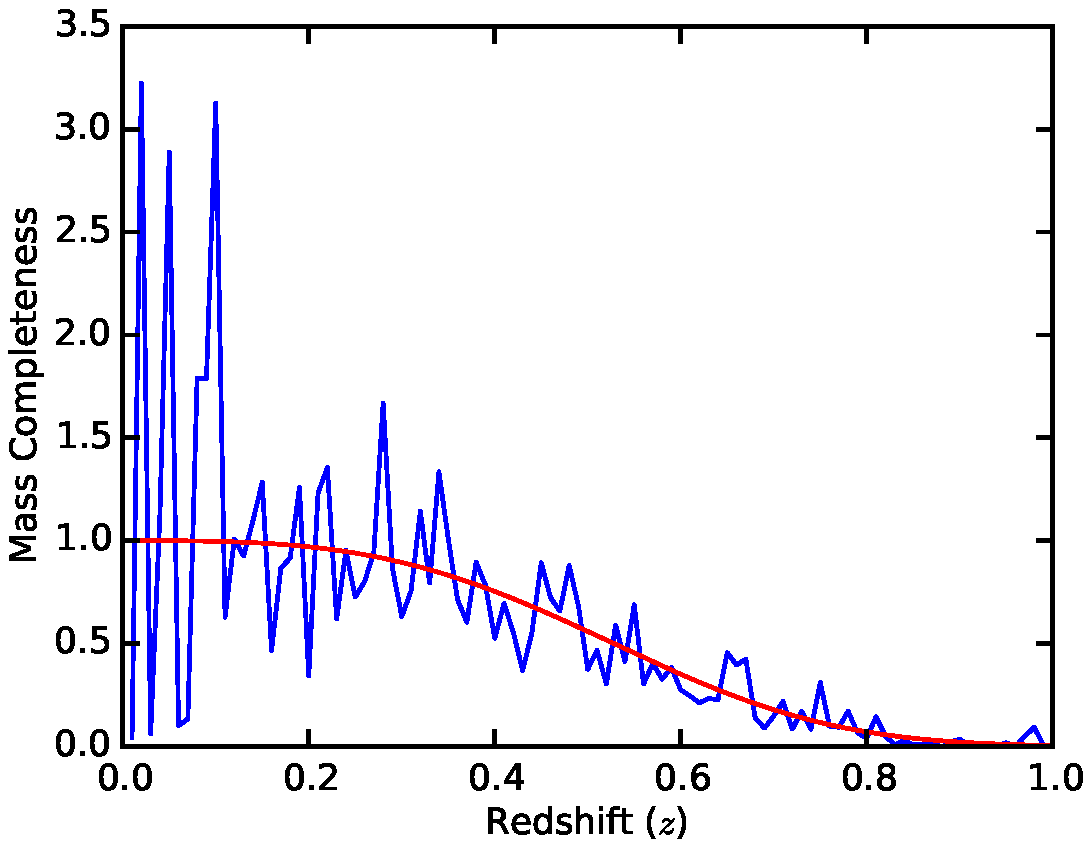
\includegraphics[width=\textwidth]{mass_completeness.pdf}
\caption{\label{fig:mass_complete} Mass completeness as a function of redshift. The blue line shows the average mass per redshift bin across the 23 fields for which we have constructed 3-D mass models. The red line shows the best fit to the data using a functional form of $f(z) = e^{-z^a / b}$ with best fit parameters $a = 3.23$ and $b = 0.183$. Because this is a fit to the average across mass models, individual beams can have higher or lower than the mean density of the universe. The only assumption is that the average of our beams should be approximately the mean density of the universe.%
}
\end{center}
\end{figure}


%%%%%%%%%%%%%%%%%%%%%%%%%%%%%%%%%%%%%%%%
\section{Which Environment/LOS Galaxies are the Most Important?}
\label{sec:Individual}
%%%%%%%%%%%%%%%%%%%%%%%%%%%%%%%%%%%%%%%%

As we have said, there may be hundreds of galaxies in our beams but they are not equally important for lensing.  Conceptually, we want to understand what properties control a perturber's influence on the lensed images.  Operationally, we need to determine whether individual perturbers should be treated as main planes or tidal planes in our framework.  In this section we use analytics and simulations to identify the combination of mass, projected offset, and redshift offset that best characterizes a perturber's significance.

\subsection{Massive Galaxies Projected Near the Lens are More Important}

We begin with the simplest case of one main lens galaxy and one perturbing galaxy in the same plane. We denote the deflection due to the main galaxy as $\al_{g}$ and the deflection due to the perturber as $\al_p$. It is useful to define the lensing potential as
\begin{equation}
\al \equiv \nabla \phi.
\end{equation}
If the perturbing galaxy does not overlap the lensed images, its gravity is the same as a point mass so we can write the lens potential as
\begin{equation}
\phi_p = R_p^2 \ln \left| \x - \vec{r} \right| 
\end{equation}
where $R_p$ is the Einstein radius of the perturber, $\x$ is the image position in the redshift plane of the perturber, and $\vec{r}$ is the position of the perturber. If we let $|\x| = x$, $|\vec{r}| = r$, and $\theta=$ the angle between the perturber and the image position as measured from the origin, we can rewrite the potential using the law of cosines as
\begin{equation}
\phi_p = \frac{1}{2}R_p^2 \ln(r^2 + x^2 - r x \cos\theta).
\end{equation}
If the perturbing galaxy is far from the lensed images, then $x \ll r$ and we can expand the potential in a Taylor series:
\begin{eqnarray}
\phi_p &=& R_p^2 \left[ \ln(r) - \cos(\theta) \frac{x}{r}  - \frac{1}{2} \cos(2\theta) \frac{x^2}{r^2} \right. \nonumber\\
&& \qquad\left. - \frac{1}{3}\cos(3\theta)\frac{x^3}{r^3}  + \ldots\right].
\end{eqnarray}
This expression can be extended beyond a point mass model as
\begin{equation}
\phi_p = \phi(0) + \alpha^i(0) x^i + \frac{1}{2}\Gamma^{ij} x^i x^j+ \frac{1}{6} \sF^{ijk} x^i x^j x^k + \ldots 
\end{equation}
where we have adopted the Einstein convention of summing over repeated indices and defined the tidal and flexion tensors:
\begin{eqnarray}
\Gamma^{ij} &\equiv& \left. \frac{\partial^2 \phi_p}{\partial x^i \partial x^j} \right|_{x=0} , \\
\sF^{ijk} &\equiv&  \left. \frac{\partial^3 \phi_p}{\partial x^i \partial x^j \partial x^k} \right|_{x=0} .
\end{eqnarray}
For a point mass, the tidal and flexion amplitudes scale as $\Gamma \propto R_p^2/r^2$ and $\sF \propto R_p^2/r^3$.

In the expansions, the zeroth order terms correspond to shifts in the zeropoint of the potential, which are unobservable.  The first order terms correspond to a uniform deflection, which can be absorbed by translating the source plane.  Therefore only the terms at second order and higher have observable consequences.

\begin{figure}[t]
\begin{center}
%crk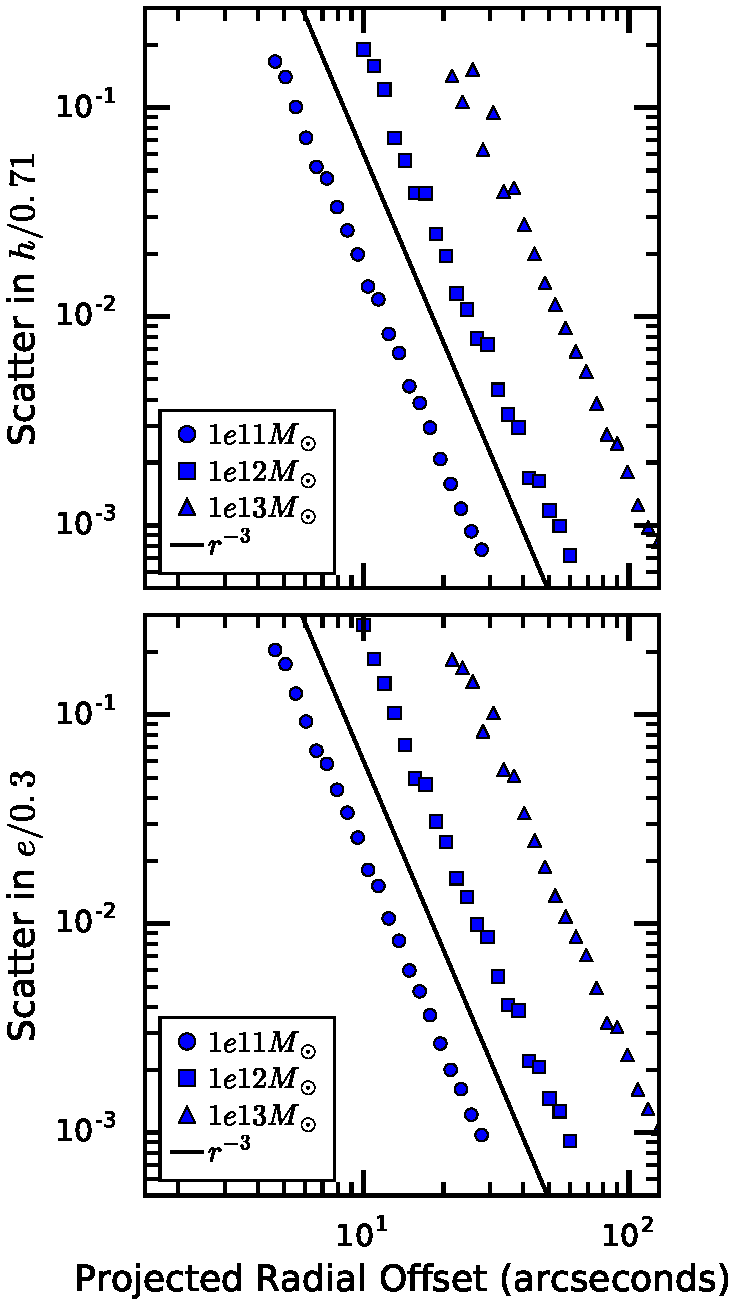
\includegraphics[width=1\columnwidth]{figures/toymass_compare/toymass_compare}
\caption{\label{fig:toyr3} Deviations in lens model parameters for simulations with a single perturbing galaxy at the same redshift as the main lens galaxy.  The horizontal axis is the radial offset of the perturber, and results are shown for three decades in mass.  Each row presents results for a different parameter: median $\chi^2$ (top), scatter in the Hubble constant ($h$, middle), and scatter in ellipticity ($e$, bottom).  Each column represents a different model: Lens-Only (left), Lens+Shear (middle), and 3-D Lens models (right). Points show results from simulations, while lines show theoretical expectations based on the following arguments.  Lens-Only models ignore even second-order terms from the perturber so we expect the scatter to scale as $r^{-2}$, while $\chi^2 \propto r^{-4}$ since it is the square of the residuals.  Lens+Shear and 3-D Lens models omit third-order terms and higher, so we expect the scatter to scale as $r^{-3}$ and hence $\chi^2 \propto r^{-6}$.  In every case, the scatter is proportional to $M \propto R_p^2$ in agreement with our theoretical expectations.%
}
\end{center}
\end{figure}

To quantify the environmental effects, we run simulations with an SIE main lens galaxy and a point mass perturber.  We choose the Einstein radius of the main lens to be $R_E = 1.0''$, and we place the lens and perturber at redshift $z_{\rm{lens}} = z_p = 0.3$ in front of a source at redshift $z_{\rm{src}} = 2.0$.  We consider three decades of perturber mass.  Figure \ref{fig:toyr3} shows the results in terms of the median $\chi^2$ value along with the scatter in the recovered values of the Hubble constant $h$ and the ellipticity $e$.

For all three of our models, the $\chi^2$ and parameter scatter increase as the perturber gets closer to the main galaxy and higher order terms become more important.  The scalings follow power laws that are consistent with our theoretical expectations.  Lens-Only models ignore even second-order terms from the perturber, and since those scale as $r^{-2}$ we expect the deviations in model parameters to follow the same scaling, while $\chi^2 \propto r^{-4}$ since it is the square of the residuals.  Lens+Shear and 3-D Lens models omit third-order terms and higher, so we expect the scatter to scale as $r^{-3}$ and hence $\chi^2 \propto r^{-6}$. Also, since the tidal and flexion amplitudes scale as $M \propto R_p^2$ we expect the parameter scatter to scale with the perturber mass.  All of these expectations are borne out by the simulations.  These results quantify our intuition that massive galaxies near the main lens are important for lensing.

\subsection{Foreground Pertubers are More Important than Background}

We now turn our attention to galaxies along the LOS. Mass that is not physically associated with lens galaxy but lies close in projection can also produce perturbations to the lens potential \citep[e.g.,][]{Bar-Kana96,Momcheva06,Wong11}. \citet{Jaroszynski14} show that omitting the effects of LOS and neighbor galaxies can often lead to unsuccessful fits, especially when time delay constraints are included.

For a single perturbing galaxy, the lens equation \ref{eqn:lenseqn} has the form
\begin{equation}
\x_2 = \x_1 - \beta_{1\,2} \al_1(\x_1)
\end{equation}
and
\begin{equation}
\x_s = \x_1 - \beta_{1\,s} \al_1(\x_1) - \beta_{2\,s} \al_2(\x_2).
\end{equation}
Combining these equations, recalling that $\beta_{i\,s} \equiv 1$, and setting $\beta \equiv \beta_{1\,2}$ lets us write the two-plane lens equation as
\begin{equation}
\x_s = \x_1 - \al_1(\x_1) - \al_2\left(\x_1 - \beta \al_1(\x_1)\right).
\label{eqn:twoplane}
\end{equation}
To make further progress, we need to distinguish situations when the perturber is in front of or behind the main lens galaxy.  In the following discussion it is useful to recall that $\beta$ varies monotonically with redshift, ranging from $\beta = 0$ when $z_p = z_{\rm{lens}}$ to $\beta = 1$ when the perturber redshift reaches either $z_p = 0$ (for a foreground perturber) or $z_p = z_{\rm{src}}$ (for a background perturber).

\subsubsection{Background Perturber}
\label{sec:background}

We begin with the case when the perturbing galaxy is in the background. The first part of this discussion parallels \citet{Keeton03}.  We have $\al_1 = \al_g$ and $\al_2 = \al_p$. Substituting this into equation \ref{eqn:twoplane} yields
\begin{equation}
\x_s = \x_1 - \al_g(\x_1) - \al_p(\x_1 - \beta \al_g(\x_1)). 
\end{equation}
We Taylor expand $\al_p$ and omit the unobservable terms corresponding to the constant potential and deflection:
\begin{eqnarray}
x^i_s &=& x^i_1 - \alpha^i_g(\x_1) - \Gamma^{ij} (x^j_1 - \beta \alpha^j_g(\x_1)) \\
&&- \frac{1}{2} \sF^{ijk} (x^j_1 - \beta \alpha^j_g(\x_1)) (x^k_1 - \beta \alpha^k_g(\x_1)) + \mathcal{O}(\x_1^4) . \nonumber
\end{eqnarray}
Here we use index notation for clarity.

If we truncate the expansion at tidal terms and return to vector/tensor notation, we can write
\begin{equation}
\label{eqn:background}
\x_s = (\I - \GammaMat) \x_1  - (\I - \beta \GammaMat)\al_g(\x_1) + \mathcal{O}(\x_1^3).
\end{equation}
This equation looks very similar to the single plane lens equation, but with some multiplicative factors. In fact, if we multiply both sides by $(\I - \beta \GammaMat)^{-1}$ from the left, introduce a scaled source coordinate $\vec{u}_{\rm eff} \equiv (\I - \beta \GammaMat)^{-1} \x_s$, and define an effective shear by
\begin{equation}\label{eqn:Geff}
\I -\GammaMat_{\rm eff} \equiv (\I - \beta\GammaMat)^{-1} (\I - \GammaMat) ,
\end{equation}
then we can rewrite equation \ref{eqn:background} as
\begin{equation}
\vec{u}_{\rm eff} = (\I - \GammaMat_{\rm eff}) \x_1 - \al_g(\x_1),
\end{equation}
which is equivalent to the single plane lens equation with an external shear in the lens plane \citep[see also][]{Schneider97}. We are allowed to rescale the source plane because the position of the source is unobservable and we typically only measure the ratio of the fluxes of different images, which is insensitive to the absolute intrinsic luminosity of the source.\footnote{The freedom to rescale the source plane vanishes if the intrinsic luminosity of the source is known.  Thus, lensed standard candles, such as type Ia supernovae \citep{Kelly15, Patel14, Kolatt98}, offer a novel way to break the mass sheet degeneracy.}

In the tidal approximation, we expect errors to be associated with the largest terms that have been neglected: the third order flexion terms.  We therefore use the terms involving $\sF$ to rank perturbers in terms of the validity of the tidal approximation.  We must make some plausible assumptions to quantify these terms.  We approximate the main lens galaxy as a singular isothermal sphere (SIS) with deflection
\begin{equation}
\al_g = R_E \rhat.
\end{equation}
Then we can write the lens equation \ref{eqn:background} in the tidal approximation as
\begin{equation}
\label{eqn:backgroundorder2}
\x_s = \x_1 - R_E \rhat -  \GammaMat (\x_1 - \beta R_E \rhat).
\end{equation}
For comparison, the lens equation with flexion terms is
\begin{multline}
\x_s = \x'_1 - R_E\rhat -  \GammaMat(\x'_1 - \beta R_E\rhat) \\
- \frac{1}{2}(\x'_1 - \beta R_E\rhat) \sF (\x'_1 - \beta R_E \rhat).
\label{eqn:backgroundorder3}
\end{multline}
where we recognize that the solutions $\x'_1$ of this equation may differ from the solutions $\x_1$ of equation \ref{eqn:backgroundorder2} because of the flexion effects.  If we assume that $\GammaMat \ll 1$ (which applies if this is truly a perturbing galaxy and not a main lens galaxy), and we subtract equations \ref{eqn:backgroundorder3} and \ref{eqn:backgroundorder2}, we can define the ``flexion shift'' caused by third order terms to be $\Delta_3 \x \equiv \x'_1 - \x_1$, and thus find
\begin{equation}
\Delta_3 \x = \frac{1}{2} (\x'_1 - \beta R_E \rhat) \sF (\x'_1 - \beta R_E \rhat).
\end{equation}
Now, if we define the perturber to be colinear with the image position ($\theta  = 0$)\footnote{If we consider all possible angles, the root mean square value has an extra factor of $\sqrt{2}$ that does not affect the scalings.} and assume that the positions of the multiple images are $|\x'_1| \approx |\x_1| \approx R_E$, we can write the magnitude of the flexion shift as
\begin{equation}
\Delta_3 x = \frac{R_E^2 R_p^2}{r^3} (1 - \beta)^2. 
\label{eqn:backgroundd3x}
\end{equation}
This flexion shift $\Delta_3 x$ has units of arcseconds. Physically this quantity corresponds to the perturbation of the image positions at the Einstein radius of the main lens caused by third order terms, a quanity that we will use to rank order the ENV/LOS contributions of perturbing galaxies.
In this derivation, we have used the expression for $\sF$ for a point mass, which is reasonable when the perturber is projected far from the images.  Strictly speaking, $r$ here is the unlensed distance in the redshift plane of the perturber. To convert to offset as observed on the sky $r'$, we use the lens equation to yield $r' = r - \beta R_E$. As long as the perturbing galaxy is many Einstein radii away from the lens, we can put $r' \approx r$.  (If that were not the case, the perturber would need to be treated as a main plane.)

\subsubsection{Foreground Perturber}
\label{sec:foreground}

The foreground case is somewhat different. Now $\al_1 = \al_p$ and $\al_2 = \al_g$, so the lens equation has the form
\begin{equation}
\x_s =\x_1 - \al_p(\x_1) - \al_g(\x_1 - \beta \al_p(\x_1)).
\end{equation}
Taylor expanding $\al_p$ yields
\begin{eqnarray}
x^i_s &=& x^i_1  - \alpha_p^i(0) - \Gamma^{ij}x^j_1 - \frac{1}{2} \sF^{ijk} x^j_1 x^k_1 +\ldots \\
&& - \alpha^i_g \left(x^i_1 - \beta\alpha_p^i(0) - \beta \Gamma^{ij} x^j_1 - \frac{1}{2} \sF^{ijk} x^j_1 x^k_1 + \ldots \right). \nonumber
\end{eqnarray}
Now truncating at tidal terms yields
\begin{equation}
\x_s = (\I - \GammaMat) \x_1 - \al_g\left((\I - \beta\GammaMat) \x_1 + \mathcal{O}(\x_1^3)\right) + \mathcal{O}(\x_1^3).
\end{equation}
This looks similar to equation \ref{eqn:background}, but there is a key difference: instead of just having a multiplicative effect on the source position like the background perturber, the deflection from the foreground perturber enters the lens equation \emph{inside the argument} of the deflection of the main galaxy. There is no way to define an effective shear that fully captures the effects of a foreground perturber (see also M14).  In principle, one can define a scaled coordinate based on the argument of the deflection to transform this equation to look like the standard lens equation \citep[e.g.,][]{Schneider97,Keeton03}. However, this requires care, as the new quantities do not correspond to the \emph{observed} image positions that are typically used in lens modeling. An alternative is to rescale the mass of the main lens galaxy to account for the change in the argument of the deflection \citep{Schneider97}, but this also requires care because the mass predicted by the lens models is no longer the true physical mass of the lens.

To examine this issue, we simulated a $10^{12} M_\odot$ perturbing galaxy at a variety of projected offsets and redshifts. To emphasize the contribution from non-linear effects, in this set of simulations we generate the mock data using the tidal approximation in our 3-D Lens framework (i.e., there are no higher order terms).  Figure \ref{fig:frontback} shows that Lens+Shear models can account for a background perturber (to within numerical precision) through an effective shear, as discussed in Section \ref{sec:background}.  By contrast, Lens+Shear models \emph{cannot} mimic the effects of a foreground LOS galaxy.  A foreground perturber has complicated effects because it creates a difference between the coordinates we see on the sky and the coordinates in the plane of the main lens galaxy.

\begin{figure}[t]
\begin{center}
%crk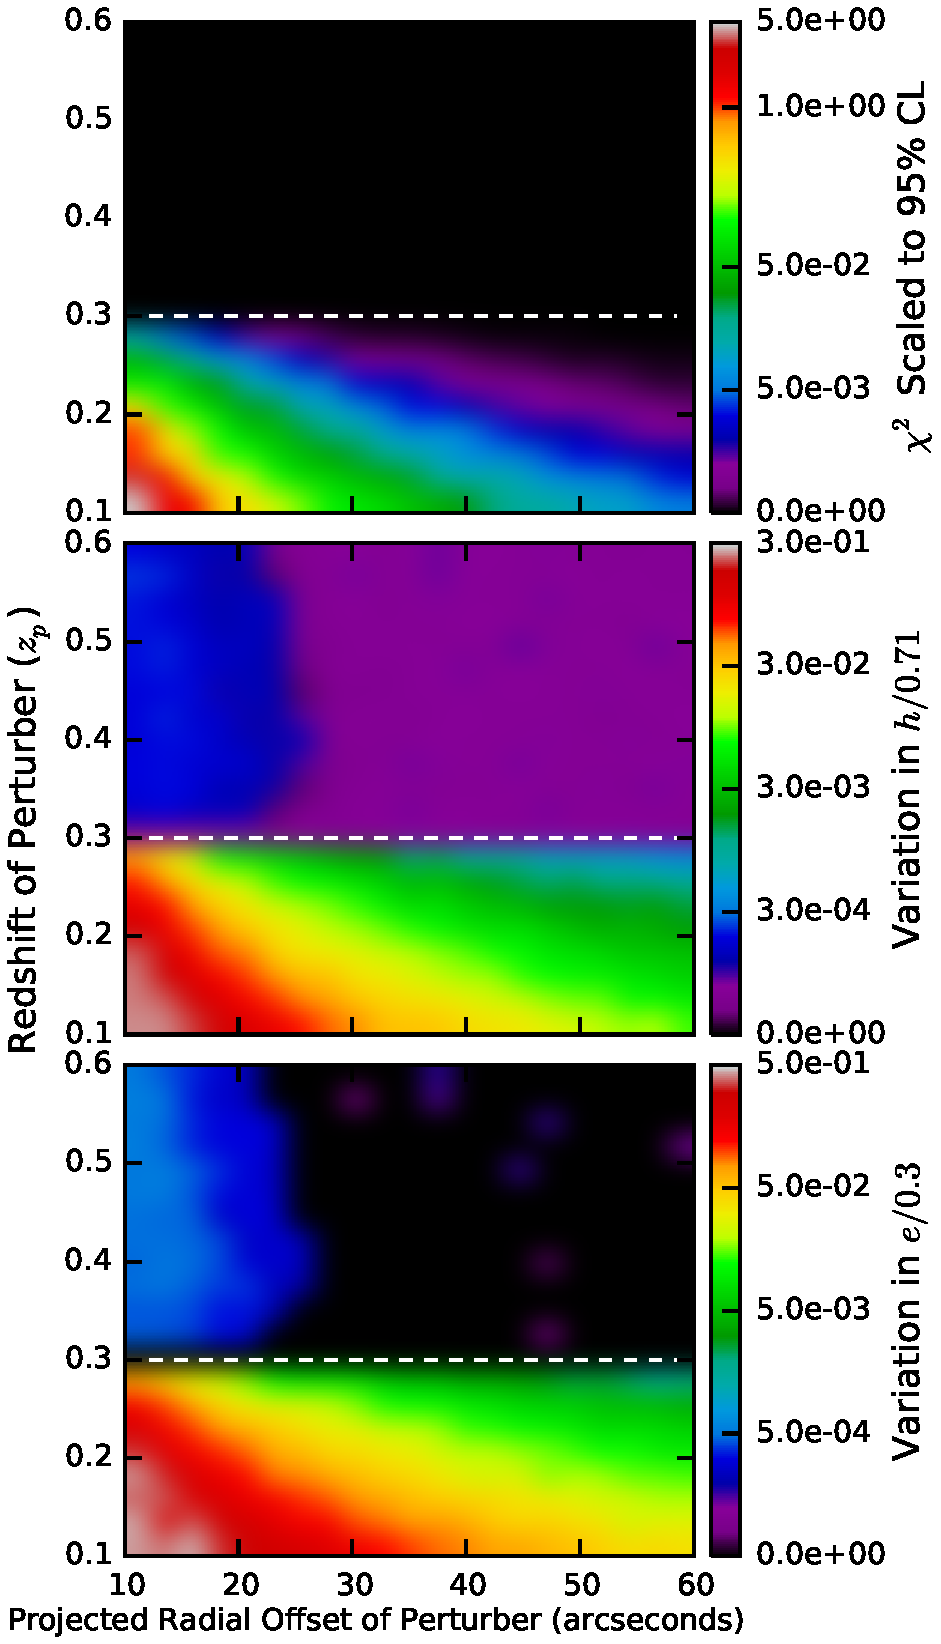
\includegraphics[width=0.7\columnwidth]{figures/mockshear/frontback}
\caption{\label{fig:frontback} Recovered lens model parameters for simulations with tidal effects from an LOS perturber.  (The simulations shown here do not include higher order terms.)  The main lens has a redshift of $z_{\rm{lens}} = 0.3$ (marked by the white dashed line) and the perturber has a mass of $10^{12}\, M_\odot$.  We use an $\asinh$ color scaling for dynamic range; at large values, $\asinh$ acts like a logarithm, but at small values, it becomes linear.  When the perturber is in the background, Lens+Shear models can use an effective shear to account for the LOS effects (see eq.\ \ref{eqn:Geff}).  When the perturber is in the foreground, however, there are non-linear effects that cannot be mimicked by a shear in the lens plane.
}
\end{center}
\end{figure}

We now seek an expression for the flexion shift $\Delta_3 x$ caused by a foreground perturber.  Following an analysis similar to that in Section \ref{sec:background}, and again using an SIS main lens and a point mass perturber, we can write the lens equation in the tidal approximation as
\begin{equation}
\x_s = \x_1 - R_E \rhat - \GammaMat(\x_1 - \beta R_E \rhat) 
\end{equation}
while the lens equation with flexion terms is
\begin{equation}
\x_s = \x'_1 - R_E \rhat - \GammaMat(\x_1 - \beta R_E \rhat) - \frac{1}{2} \x_1 \sF \x_1.
\end{equation}
Subtracting these equations and rearranging yields
\begin{equation}
\Delta_3 \x = \frac{1}{2} \x_1 \sF \x_1.
\end{equation}
In this case, the multiple images form at $\x_2 \approx R_E \rhat$, implying that $R_E \approx \x_1 - \beta \GammaMat \x_1$. If we assume that $\GammaMat \ll 1$ (as above), we can write $\x_1 \approx R_E \rhat$, giving
\begin{equation}
\Delta_3 x = \frac{R_E^2 R_p^2}{r^3}.
\label{eqn:foregroundd3x}
\end{equation}
This equation is similar to equation \ref{eqn:backgroundd3x}, but without any $\beta$ factors. Therefore, not only can foreground perturbers not be mimicked by an external shear because of non-linear effects, but they also have a different weighting than background perturbers.

\subsubsection{Implications}

\begin{figure}[t]
\begin{center}
%crk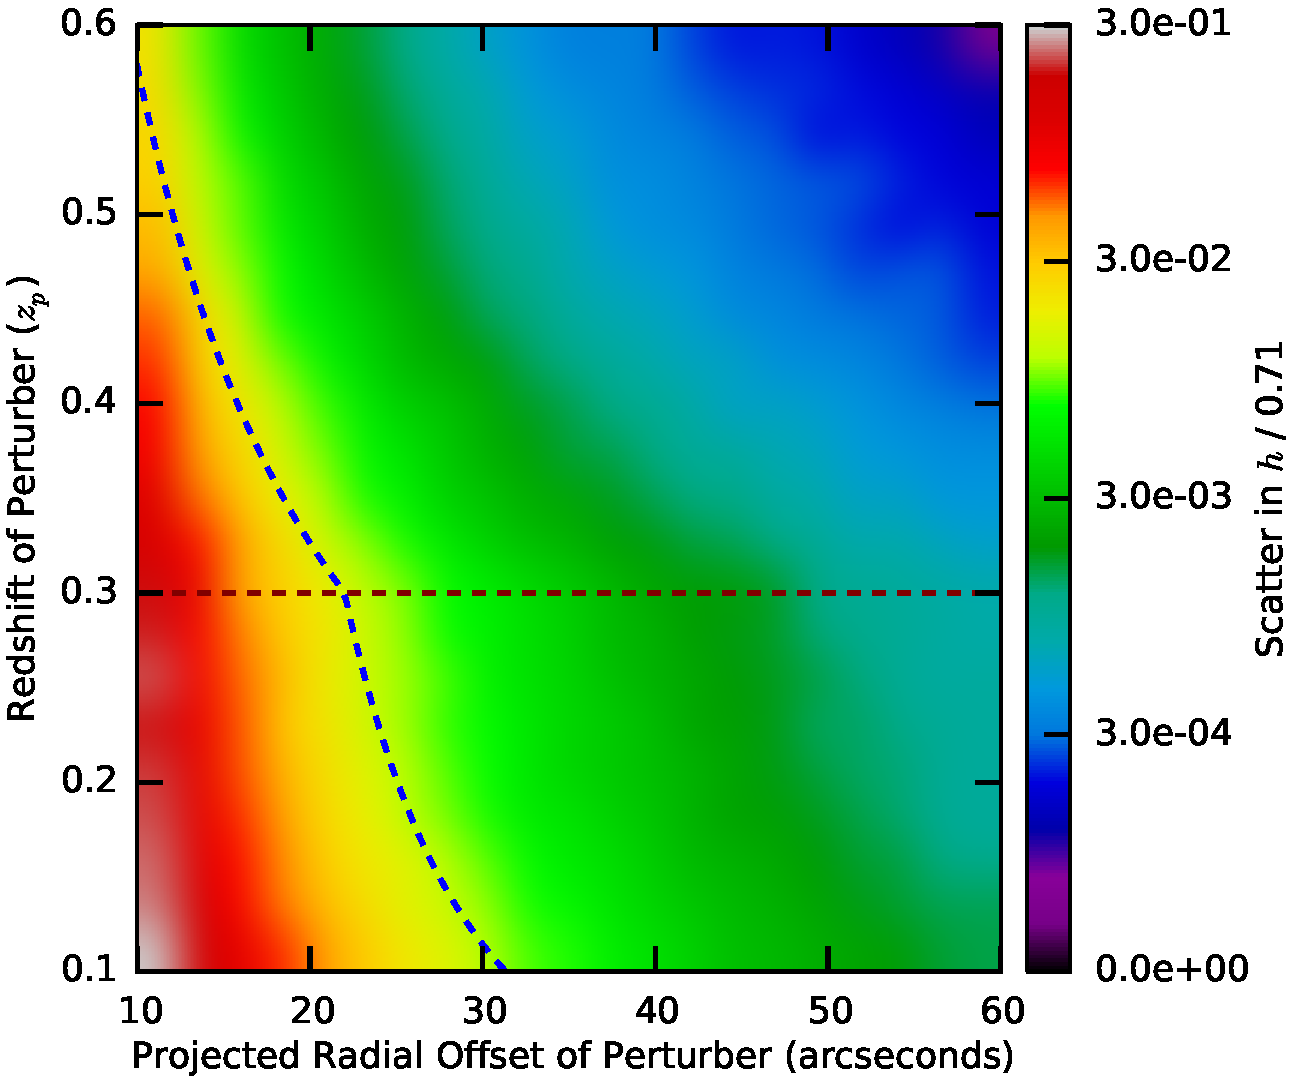
\includegraphics[width=0.98\columnwidth]{figures/toyh/toyh}
\caption{\label{toyhd3x} Scatter in the Hubble constant, $h$, recovered from 3-D Lens models for perturbers at different projected offsets and redshifts.  The main lens has a redshift of $z_{\rm{lens}} = 0.3$ which is marked with a dotted line, and the perturbing galaxy has a mass of $10^{12}\,M_\odot$.  The dashed line shows a contour of constant flexion shift, $\Delta_3 x$, from equations \ref{eqn:backgroundd3x} and \ref{eqn:foregroundd3x} (picking a different value of $\Delta_3 x$ would simply rescale the contour).  The curve matches the shape of the color contours, indicating that our theoretical expression captures the redshift dependence of LOS effects.  Thus, we can use the flexion shift to compare effects of LOS galaxies even if they are at different redshifts.
}
\end{center}
\end{figure}

We now use simulations to test whether our expression for the flexion shift $\Delta_3 x$ (eqs.\ \ref{eqn:backgroundd3x} and \ref{eqn:foregroundd3x}) provides a useful way to characterize the importance of LOS perturbers.  We fix the perturber mass to be $10^{12}\,M_\odot$ but vary its projected offset and redshift.  For each scenario we generate mock lenses and then fit them using 3-D Lens models in the tidal approximation.  We treat the perturber as a point mass, which is not a valid assumption when the projected offset or redshift is small, but is reasonable in the regime where we anticipate using the tidal approximation.  Figure \ref{toyhd3x} shows the scatter in the recovered value of the Hubble constant (the median value is not shown because it matches the input value; there is no bias).  Generally speaking, the scatter increases as the offset decreases and higher order terms become more significant.  There is a complicated redshift dependence: in the background, the perturber's effects become weaker as the redshift offset increases because of the $\beta$ factors in equation \ref{eqn:backgroundd3x}; while in the foreground, the perturber's effects become stronger as $z \to 0$ because its angular Einstein radius increases.  Both of these scalings are well described by our functional form for $\Delta_3 x$.

\begin{figure}[t]
\begin{center}
%crk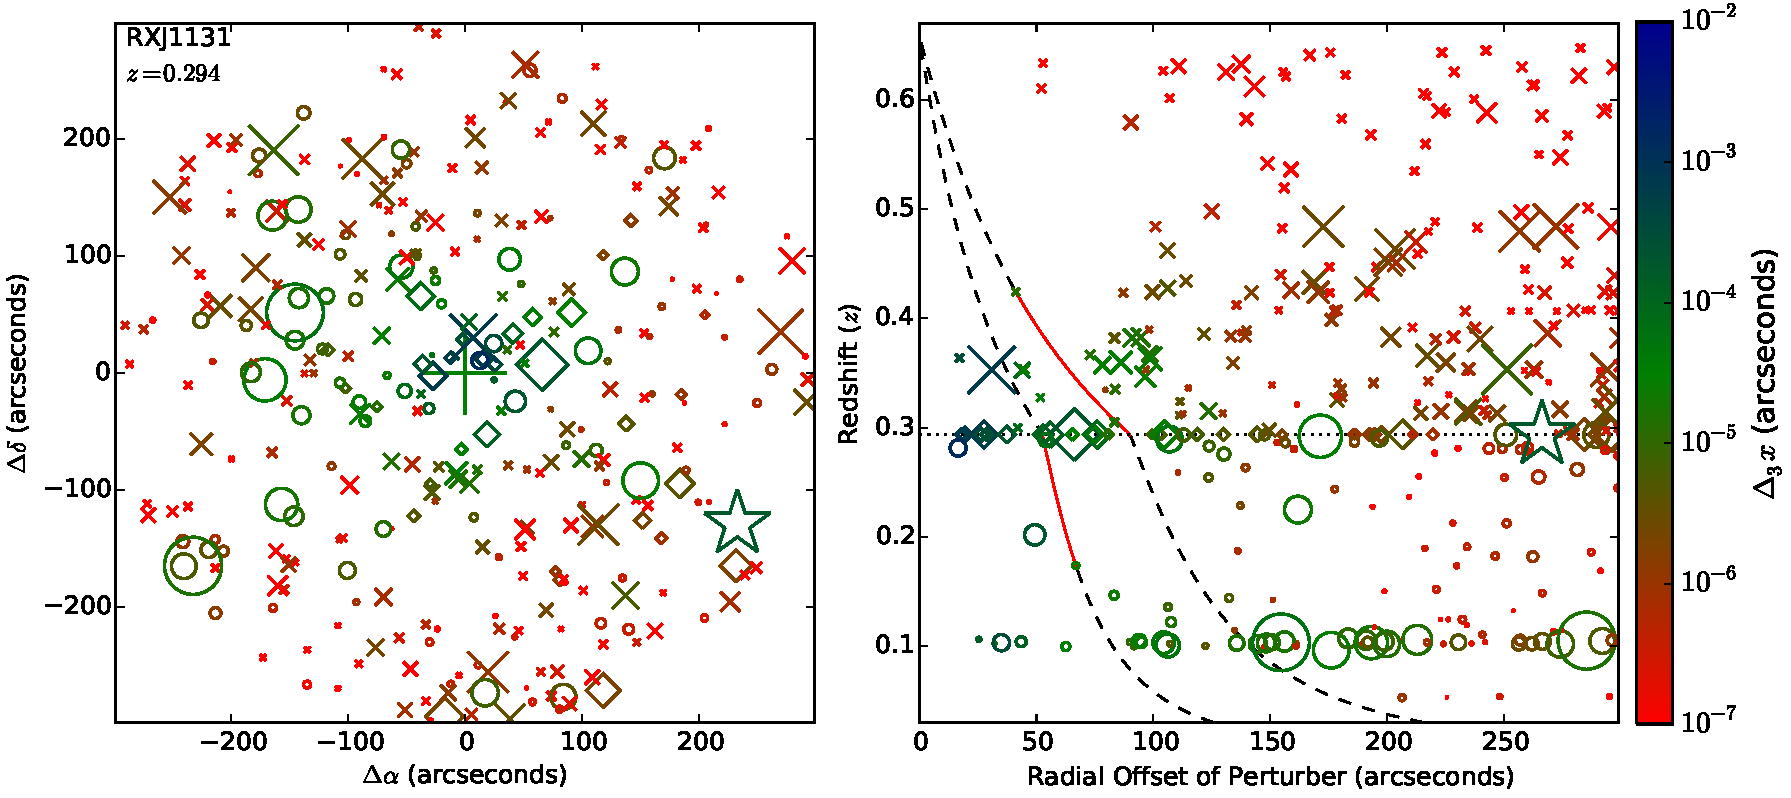
\includegraphics[width=1\columnwidth]{figures/B0712_fieldrz/RXJ1131_fieldrz}
\caption{\label{fig:fieldrz} Illustration of the flexion shift for galaxies in the field of RXJ1131.  In the left panel, each galaxy is shown at its position on the sky.  The area of each point is proportional to the mass of the galaxy.  X's and O's mark galaxies behind and in front of the main lens galaxy, respectively, while diamonds mark members in the group around the main lens, and the star indicates the location of the common group halo.  The color of the points represents the strength of the lensing effects measured by $\Delta_3 x$. The right panel shows the same galaxies plotted in the $r$-$z$ projection. The main lens redshift is indicated by the dotted line. Two $\Delta_3 x$ contours have been shown to guide the eye. The red section of the contour illustrates how to map a perturbing galaxy to its effective offset as if it were in the main lens plane. That that there is no simple radial cut that selects the most important LOS galaxies; a more complicated quantity like $\Delta_3 x$ is necessary.%
}
\end{center}
\end{figure}

Many lens systems have significant contributions from in their local environment, (e.g. HE0435-1223 has a neighbor \citealt{Kochanek06}; MG0414+0534 \citep{Tonry99}, RXJ1131$-$1231 \citep{Sluse03}, and B2114+022 \citep{King99} all have satellites that are presumably close enough to matter), and while some models do treat nearby perturbers exactly \citep[e.g.][]{Fadely12}, typically the decision whether to include a neighbor galaxy in a model is \textit{ad hoc}. The flexion shift, $\Delta_3 x$, provides a quanitative criterion to compare the importance of LOS galaxies even if they are at different redshifts. Therefore we can use the flexion shift to  Any given perturber can be treated with the tidal approximation if its $\Delta_3 x$ value is small, but it must be treated explicitly if its $\Delta_3 x$ value is large.  Before quantifying the threshold for ``large'' versus ``small'' (see Section \ref{sec:los_vs_shear}), it is useful to examine the range of $\Delta_3 x$ values in typical lens fields.  We consider the system RXJ1131$-$1231 (hereafter RXJ1131, e.g. \citealt{Suyu13}), which has a source at redshift $z_{\rm{src}} = 0.658$ and a lens in a group at redshift $z_{\rm{lens}} = 0.2936$.  We adopt an Einstein radius of $R_E = 1.5''$, close to the measured value \citep{Suyu13} and also close to the peak of the observed distribution \citep{Sonnenfeld13}, and an ellipticity of $e=0.3$.  Figure \ref{fig:fieldrz} illustrates $\Delta_3 x$ values for galaxies in this field.  While $\Delta_3 x$ generally increases toward the lens, there is no single radial cut that can be used to determine the importance of a perturber because perturber mass and redshift must also be taken into account.  By following contours of constant $\Delta_3 x$, as illustrated in right-hand panel, we can determine the effective radial offset for the perturber if it were in the main lens plane. Since background perturbers are downweighted by ($1-\beta)^2$, they must have a smaller projected offset to have the same effect as if they were in the main lens plane. 

\begin{figure}[t]
\begin{center}
%crk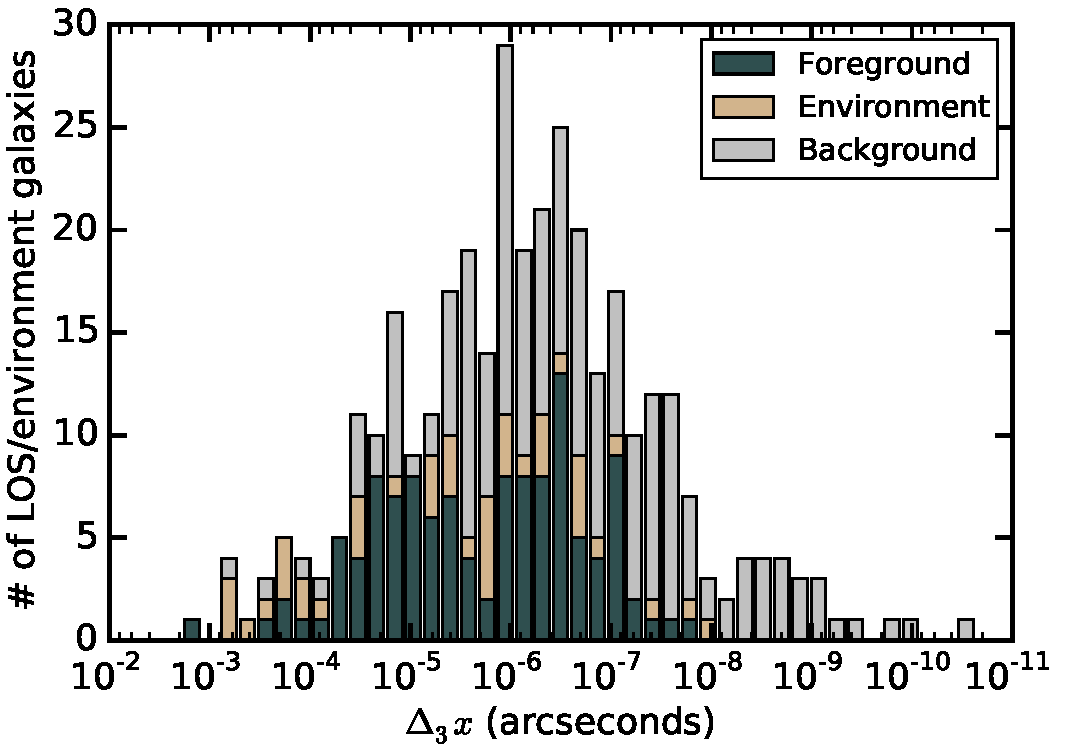
\includegraphics[width=0.7\columnwidth]{figures/RXJ1131_dx3_hist/RXJ1131_dx3_hist}
\caption{\label{fig:d3xhist} Histogram of flexion shifts for galaxies in the field of RXJ1131.  The dark (light) gray bins represent perturbing galaxies in the foreground (background) of the main lens galaxy, while the silver bins in between correspond to group members in the immediate environment of the main lens. As anticipated, foreground perturbers and group members tend to have larger $\Delta_3 x$ values than background perturbers.%
}
\end{center}
\end{figure}

Figure \ref{fig:d3xhist} shows a histogram of all the $\Delta_3 x$ values for this field.  The flexion shifts range from $\sim 5 \times 10^{-3}$ arcseconds down to $<10^{-10}$ arcseconds, with background perturbers generally having smaller values than foreground perturbers or group members.  In the next section we consider the quantitative threshold for $\Delta_3 x$ needed to achieve desired accuracy and precision in lens model results.


%%%%%%%%%%%%%%%%%%%%%%%%%%%%%%%%%%%%%%%%
\section{External Shear vs.\ 3-D Lensing}
\label{sec:los_vs_shear}
%%%%%%%%%%%%%%%%%%%%%%%%%%%%%%%%%%%%%%%%

Now that we understand how to assess the significance of different perturbing galaxies, we are ready to quantify ENV/LOS effects in realistic beams containing hundreds of galaxies.  We generate mock lens data using the full 3-D mass models in the simulations described in Section \ref{sec:setup}.  We then examine how well lens model parameters can be recovered by our 3-D lens models (which adopt the tidal approximation but keep the 3-D mass structure) or by models that make even stronger assumptions, neglecting redshift effects (Lens+Shear) or ignoring external matter altogether (Lens-Only).  In this section we focus on the field of RXJ1131.  As noted in Section \ref{sec:setup}, we combine results for 300 mock quad lenses with different source positions and azimuthal angles for the main lens galaxy.

\begin{figure}[t]
\begin{center}
%crk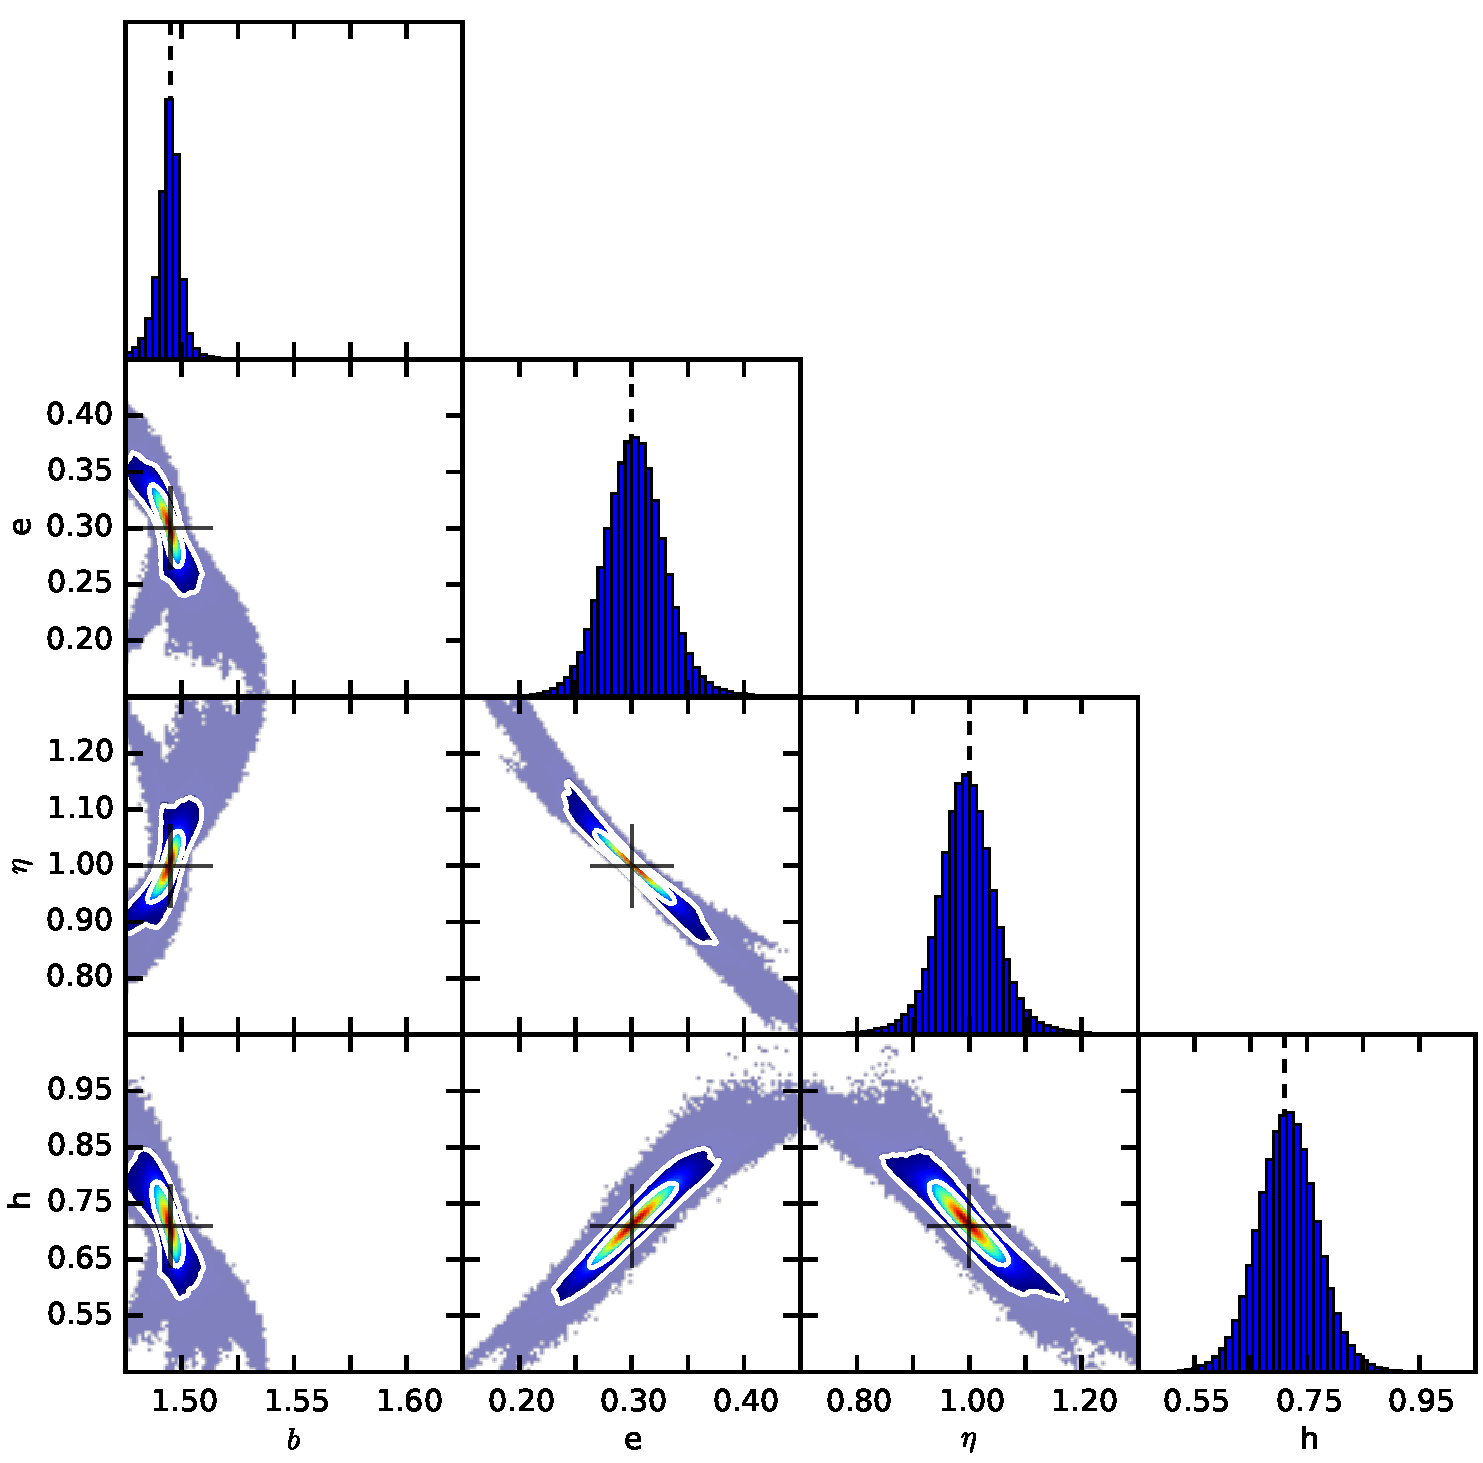
\includegraphics[width=1\columnwidth]{figures/all_los_1e-1/all_los_1e-2}
\caption{\label{fig:los_triangle} Posterior distributions for model parameters from 3-D Lens models fit to mock quad lenses in the field of RXJ1131.  The true input values are marked with crosses.  Here all perturbing galaxies are treated with the 3-D tidal approximation.  We combine MCMC results for 300 mock lenses with different source positions and azimuthal angles for the main lens galaxy.  Contours containing $68\%$ and $95\%$ of the MCMC trials are shown in white. There is no bias in the recovered parameters. However, there are strong correlations between ellipticity, the power law index, and the Hubble constant. This is a manifestation of the lens profile degeneracy \citep{Kochanek02}. The plotting ranges for corresponding parameters are the same as Figures \ref{fig:shear_triangle} and \ref{fig:scaled_triangle} to facilitate direct comparison.%
}
\end{center}
\end{figure}

We start with 3-D lens models in which the threshold on the flexion shift is large enough that all perturbing galaxies are treated with the tidal approximation.  Figure \ref{fig:los_triangle} shows posterior distributions for lens model parameters including the mass normalization (which is related to the Einstein radius; see eq.\ \ref{eqn:powerlaw}), ellipticity, power law index, and Hubble constant.  There is no bias in any of the parameters recovered from these models, but there are strong correlations among the ellipticity, power law index, and Hubble constant that we discuss momentarily.

\begin{figure}[t]
\begin{center}
%crk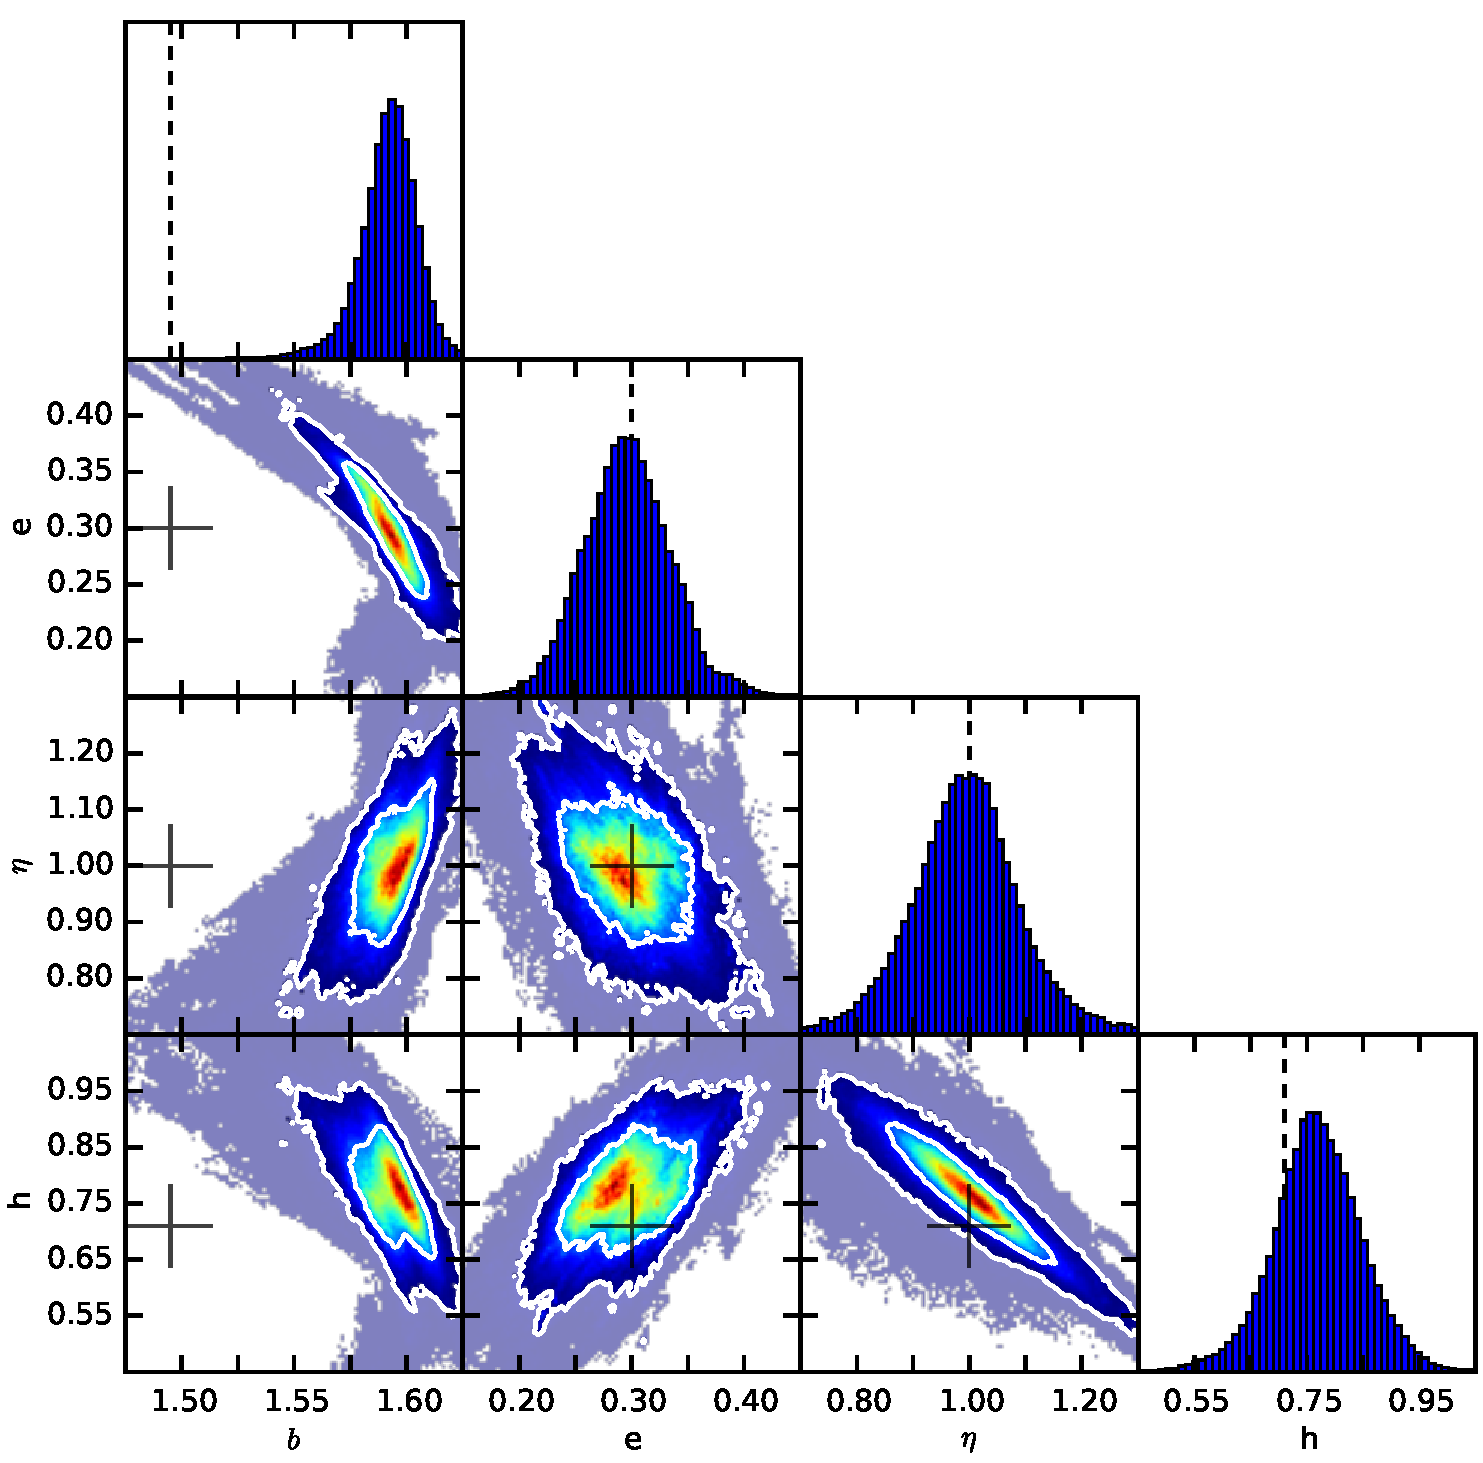
\includegraphics[width=1\columnwidth]{figures/all_shear_1e-3/all_shear_1e-2}
\caption{\label{fig:shear_triangle} Similar to Figure \ref{fig:los_triangle}, but for Lens+Shear models.  Many of the parameters show biases that were not present in 3-D lens models; most notably, the Einstein radius parameter ($b$) is strongly biased because Lens+Shear models do not explicitly include external convergence (such models must add external convergence in post-processing).  In general, the parameter distributions for Lens+Shear models are broader and more complex than they are for the 3-D Lens models shown in \ref{fig:los_triangle}.  The lens profile degeneracy is still present.%
}
\end{center}
\end{figure}

Figure \ref{fig:shear_triangle} shows comparable results for Lens+Shear models.  These models show more scatter than the 3-D Lens models, but more importantly they have biases that are most dramatic in the Einstein radius and Hubble constant.  The bias in Einstein radius is due to external convergence and will be discussed in more detail below.  The Lens+Shear models show similar correlations among $e$, $\eta$, and $h$ as in 3-D Lens models, but overall the parameter distributions are considerably more complicated and show some evidence of multiple families of best fit models.

The correlations involving the Hubble constant are associated with the ``lens profile degeneracy'':  there can be a range of density profiles that all yield a good fit but lead to different values for $h$.  \citet{Kochanek02} shows that to lowest order the degeneracy is characterized by the scaling $h \propto 1 - \langle \kappa \rangle$ where $\langle \kappa \rangle$ is the average convergence from the main lens in the annulus between the image positions.  If we assume that the image annulus is narrow and centered on the Einstein radius, we can evaluate the angle average as
\begin{equation}
\langle \kappa \rangle = \frac{1}{2 \pi} \int_{0}^{2 \pi} \kappa(R_E, \theta) d \theta.
\end{equation}
With our power law model (eq.\ \ref{eqn:powerlaw}), we can evaluate the integral by making a Taylor series expansion in the ellipticity and using
\begin{equation}\label{eqn:e-series}
\int_0^{2 \pi} \frac{d \theta}{ (1 - 2 e \cos^2(\theta) + e^2\cos^2(\theta))^{1 - \eta / 2}} \approx 1 + e  - \frac{ e \eta}{2}.
\end{equation}
For typical parameter values of interest, we find numerically that this approximation is good to $\sim1\%$.  Then we can approximate the average convergence at the Einstein radius as
\begin{equation}\label{eqn:kappa-avg}
\langle \kappa \rangle \approx \frac{1}{2} \eta  (1 - e)^{2 - \eta} \left(1 +  e - \frac{e \eta }{2}\right).
\end{equation}
We test this analysis by plotting $h/(1-\langle\kappa\rangle)$ in Figure \ref{fig:scaled_triangle}.  Most of the correlation of $h$ with $\eta$ and $e$ has been accounted for.  Remaining correlations are likely due to higher order terms in the expression for $h$ as a function of profile parameters \citep{Kochanek02} and the Taylor series expansion in equation \ref{eqn:e-series}.

\begin{figure}[t]
\begin{center}
%crk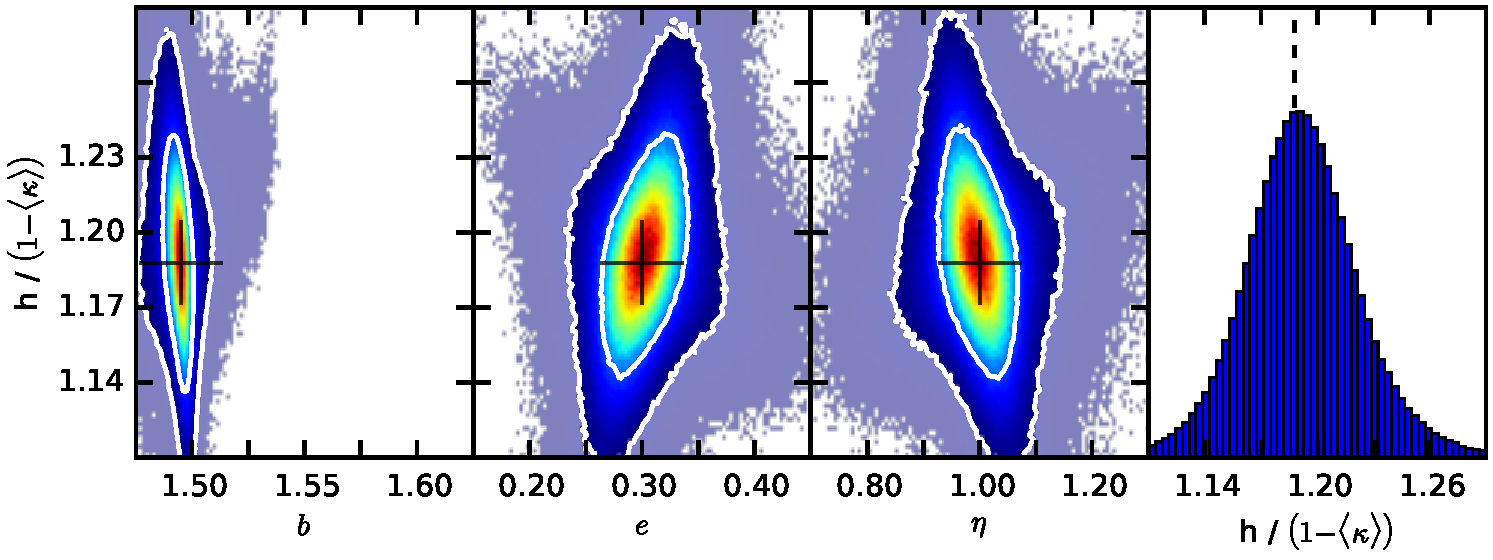
\includegraphics[width=1\columnwidth]{figures/los_scaled_h1/los_scaled_h}
\caption{\label{fig:scaled_triangle} Recovered parameter distributions for 3-D Lens models (q.v.\ Fig.\ \ref{fig:los_triangle}), but now with the Hubble constant, $h$, scaled to account for the lens profile degeneracy.  We approximate the average convergence at the Einstein radius using equation \ref{eqn:kappa-avg}. The correlations among the Hubble constant, ellipticity, and power law index are mostly removed. The residual correlations are likely due to higher order terms in the expression for $h$ \citep{Kochanek02} and the Taylor series expansion for $\langle \kappa \rangle$.%
}
\end{center}
\end{figure}

Our next goal is to determine when it is valid to use the tidal approximation.  We want to find a sweet spot that speeds up the modeling without introducing systematic uncertainties that are larger than the measurement uncertainties.  Figure \ref{fig:RXJ1131} shows results from 3-D Lens model fits with different cuts on the flexion shift, $\Delta_3 x$.  Each point on the horizontal axis corresponds to a different \emph{threshold} for $\Delta_3 x$: galaxies with larger flexion shifts are treated exactly, while galaxies with smaller values are treated with the tidal approximation.  (Note that the threshold \emph{decreases} from left to right in the plot; at a given point, galaxies to the left are exact perturbers while galaxies to the right are tidal perturbers.)  The error bars mark the $16^{th}$ and $84^{th}$ percentiles of the posterior distribution for the lens model parameters.  Our modeling uses MCMC methods to obtain posterior distributions, so the errorbars correspond to marginalized single-parameter posteriors.

\begin{figure}[t]
\begin{center}
%crk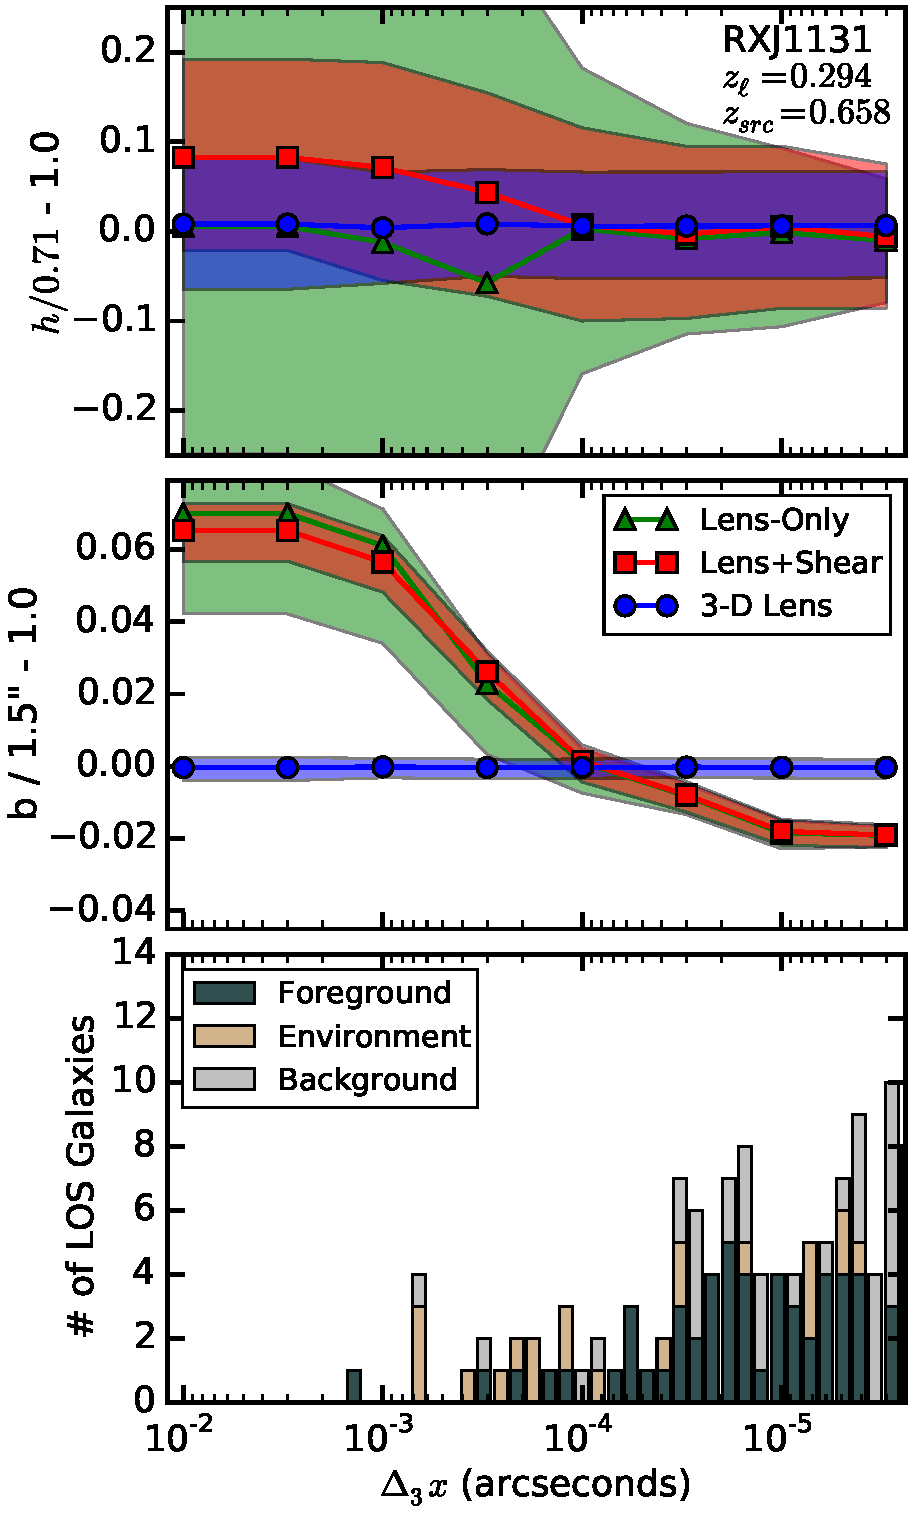
\includegraphics[width=0.7\columnwidth]{figures/B0712/new_RXJ1131_reallos}
\caption{\label{fig:RXJ1131} Results for lens models with different thresholds for the tidal approximation, using the RXJ1131 field.  For a given value of $\Delta_3 x$, we run models in which all perturbing galaxies with a larger value of the flexion shift (i.e., those toward the left in the bottom panel) are treated exactly, while perturbing galaxies with a smaller value of the flexion shift (i.e., those toward the right) are treated with the tidal approximation.  Starting at the left, all perturbers are tidal (as in Figs.\ \ref{fig:los_triangle} and \ref{fig:shear_triangle}); moving to the right increases the number of perturbers that are treated explicitly instead.  The top panel shows the median and 68\% confidence interval for the Hubble constant recovered from 3-D Lens models (blue), Lens+Shear models (red), and Lens-Only models (green).  The middle panel shows similar results for the Einstein radius parameter.  The scatter is driven by the lens profile degeneracy.  Lens-Only and Lens+Shear models tend to be biased because of external convergence effects (see text).%
}
\end{center}
\end{figure}

The first result from Figure \ref{fig:RXJ1131} is that 3-D Lens models do not show any bias in key parameters, at least for the RXJ1131 field.  It is not fully apparent given the scale of the figure, but the scatter in model parameters decreases a little as the $\Delta_3 x$ threshold is reduced and the strongest perturbers are incorporated into the model explicitly.  We believe that it is worthwhile to set a conservative threshold of $\Delta_3 x \sim 10^{-4}$ arcseconds (i.e., 1.5 dex smaller than our astrometric uncertainties), which amounts to including the strongest 10--15 perturbers explicitly.  The computational cost is not prohibitive, since the vast majority of the $\sim 300$ galaxies in the beam are still treated with the 3-D tidal approximation.

By contrast, Lens+Shear and Lens-Only models can be biased by as much as $\sim 7\%$ in the Einstein radius.  The bias is associated with external convergence: the total mass in the simulated lenses includes contributions from the environment and LOS; if we assign all of that mass to the main lens galaxy (as in Lens+Shear and Lens-Only models), we overestimate the galaxy's mass and Einstein radius.  In the traditional approach, external convergence must be included through post-processing \citep{Collett13, Suyu10}.  In our approach, introducing a few of the strongest perturbers (i.e., moving to the right in the figure) means that we begin to build up a physical model for the sources of external convergence, which reduces the bias.  In principle, there is a point at which the sources of convergence are properly accounted for and the bias is removed.  In practice, that point is not easy to determine \emph{a priori}.  Going to very small values of $\Delta_3 x$ (i.e., far to the right in the figure) actually leads to a negative bias.  This is because Lens-Only and Lens+Shear models do not include the void correction discussed in Section \ref{sec:Voids}.  Apparently the void correction is approximately 2\% in the Einstein radius for the RXJ1131 field.

Our 3-D Lens models avoid such biases because, rather than treating shear and convergence separately, we build a self-consistent physical model and then extract both the shear and convergence from it. We favor this approach because shear and convergence arise from the same underlying mass distribution and are therefore not independent.

\citet{Wong11} also showed that fitted shear parameters from the Lens+Shear models did not match the effective shear derived from the 3-D mass models. In Figure \ref{fig:shear_compare}, we show the contours for the fitted shear, while the input effective shear is shown as cross. The peak of the fitted distribution is $\sim 2\sigma$ away from the truth, broadly consistent with the results found in \citet{Wong11}. While a detailed analysis of this effect is beyond the scope of this work, the results in Figure \ref{fig:shear_compare} are suggestive that non-linear terms (due to foreground perturber) could explain the discrepancy between fitted shear and the effective shear from the ENV/LOS.

\begin{figure}[t]
\centering
%\includegraphics{figures/shear_compare.pdf}
\caption{Marginalized posterior distribution of fitted external shear values from the Lens+Shear models. $1\sigma$ and $2\sigma$ contours are shown in white. The effective shear calculated from the input 3-D mass model is shown with an orange cross. The peak of the distribution from the MCMC models is $\sim 2 sigma$ away from the truth, similar to what was found by \citet{Wong11}. The offset is likely due to non-linear effects from foreground perturbering galaxies.}
\label{fig:shear_compare}
\end{figure}

%%%%%%%%%%%%%%%%%%%%%%%%%%%%%%%%%%%%%%%%
\section{Diversity Among Lensing Beams}
\label{sec:Environments}
%%%%%%%%%%%%%%%%%%%%%%%%%%%%%%%%%%%%%%%%

So far, we have presented results for a single lens field.  In order to understand whether our conclusions are general, we need to examine how ENV/LOS effects vary from one lensing field to another.

\begin{figure}[t]
\begin{center}
%crk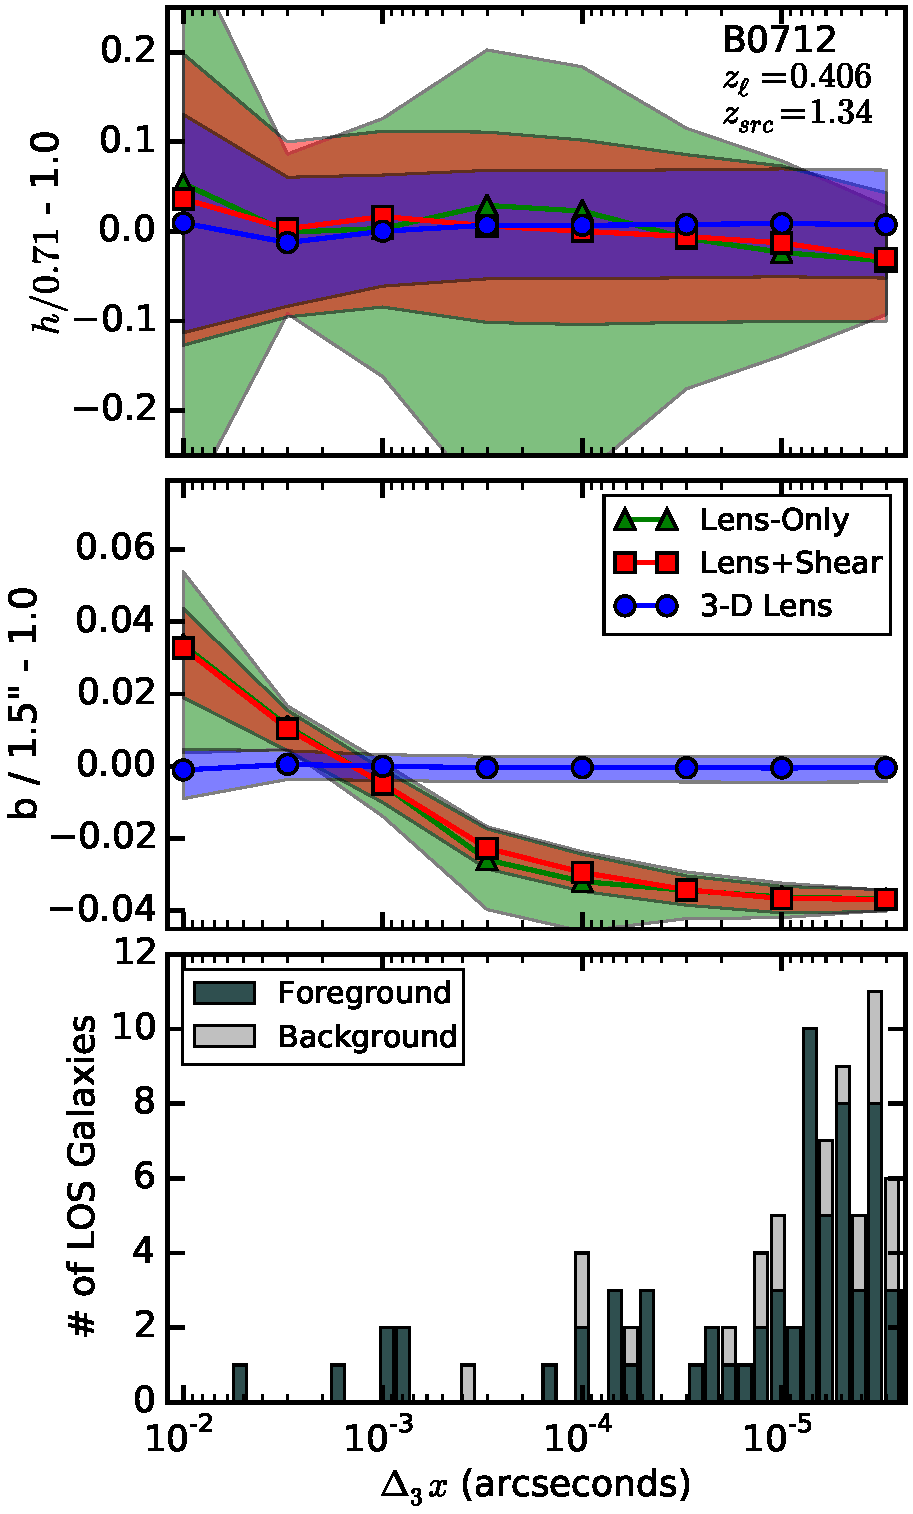
\includegraphics[width=0.7\columnwidth]{figures/B1422/new_B0712_reallos}
\caption{\label{fig:B0712} Similar to Figure \ref{fig:RXJ1131}, but for the B0712 field.  This field has a group of galaxies along the LOS to the main lens.  The qualitative trends from LOS effects are similar to what we saw before, but the quantitative details differ.%
}
\end{center}
\end{figure}

One simple test is to compare models that use the same fiducial main lens galaxy ($R_E = 1.5\arcsec$ and $e=0.3$) but different fields.  Whereas before we used the field of RXJ1131, now we consider B0712+472 (hereafter B0712; \citealt{Jackson98}).  Figure \ref{fig:B0712} shows the new results.  The trends are similar to what we saw for RXJ1131 in Figure \ref{fig:RXJ1131}, but the deviations are somewhat smaller here.  This is because the main lens in B0712 is not part of a group, although there is a group that is offset in both projection and redshift.  The correction due to voids is larger for B0712 at $\sim4\%$.

\begin{figure}[t]
\begin{center}
%crk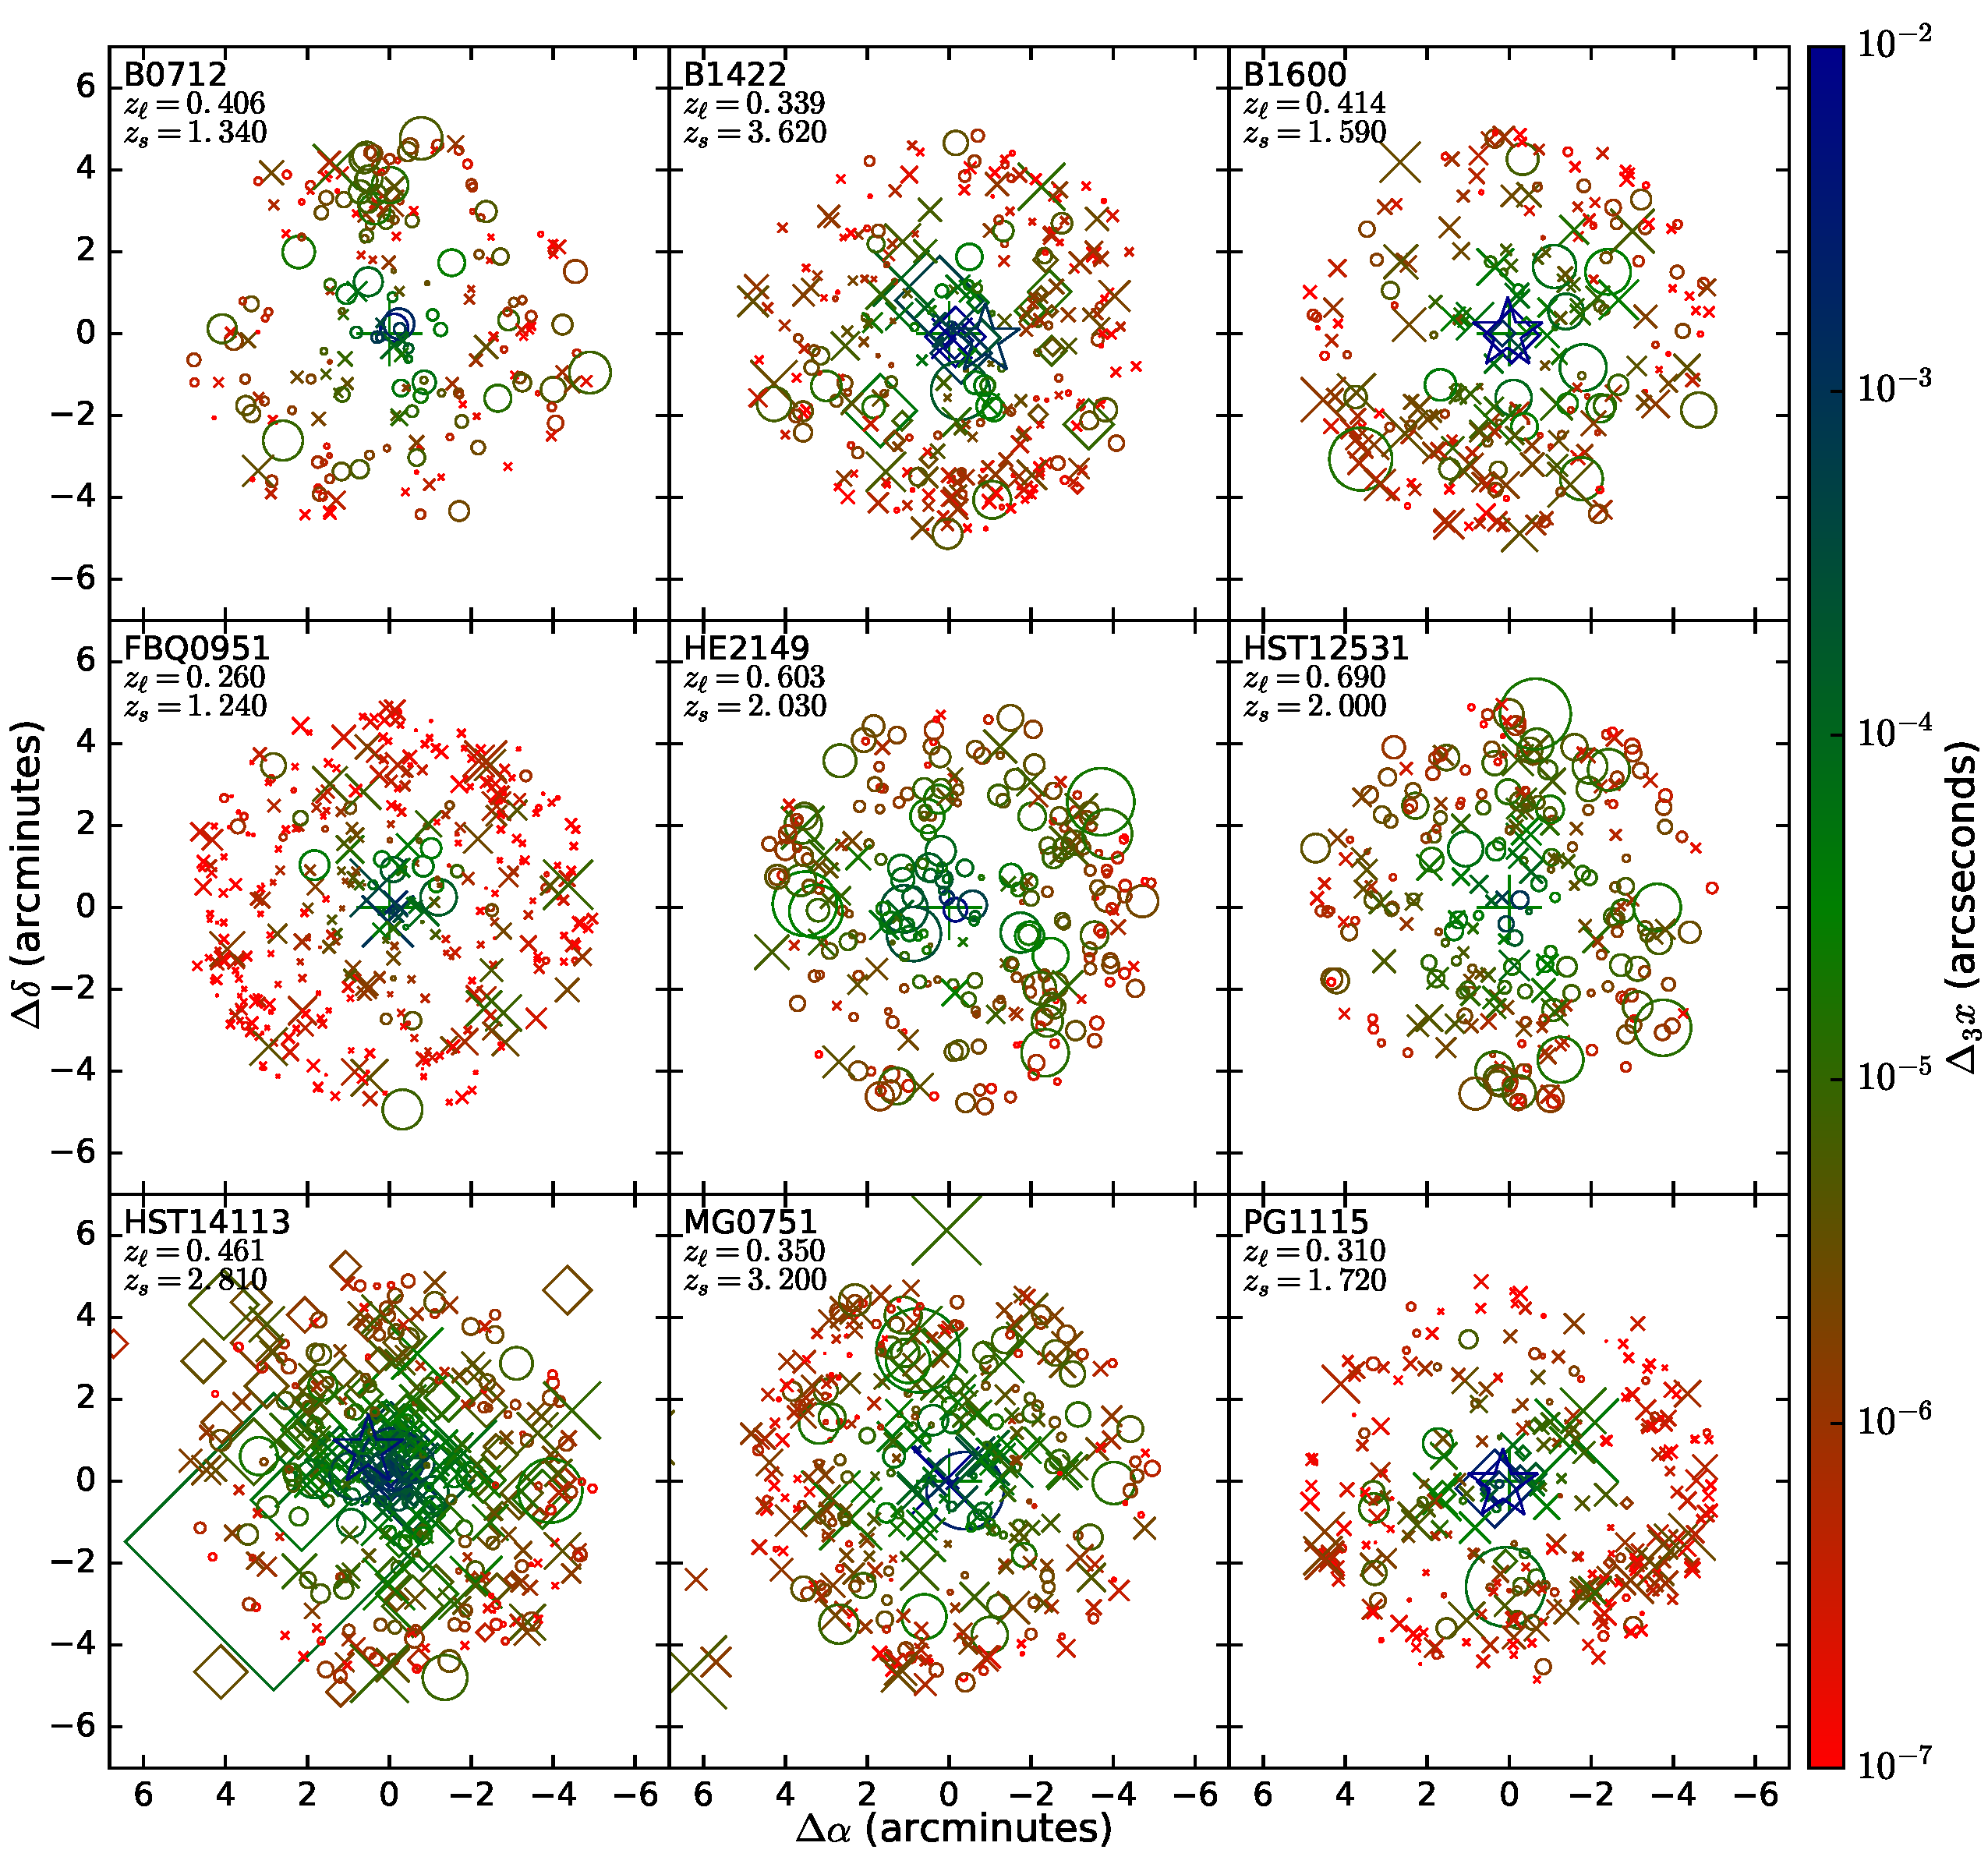
\includegraphics[width=1\columnwidth]{figures/allfields/allfields}
\caption{\label{fig:allfields} Illustration of the flexion shifts, $\Delta_3 x$, for perturbing galaxies in nine lens fields (similar to the left panel in Fig.\ \ref{fig:fieldrz}). Each galaxy in the mass model is shown in projection on the sky. The area of each point is proportional to the mass of the galaxy. X's are behind the main lens galaxy, while O's are in the foreground. Diamonds represent group members, while stars indicate the locations of group halos. The color of the points represents the strength of the higher order terms characterized by $\Delta_3 x$. There is dramatic variation in the ENV/LOS strengths across the different fields, implying that each field needs to be treated on an individual basis.%
}
\end{center}
\end{figure}

We can also characterize values of the flexion shift for a wider range of fields.  Figure \ref{fig:allfields} shows $\Delta_3 x$ values for nine other multiply-imaged QSO fields from \citet{Wong11}.  The fields are all complex; there is not a simple radial cut that divide the sample into exact and tidal perturbers.  There is striking diversity in the strength of external effects.  Fields that have groups tend to have more galaxies with high $\Delta_3 x$ values. There is no single number of galaxies that is guaranteed to be be the ``right'' number to include in lens models.  Each field must be considered on an individual basis.


\begin{figure}[t]
\centering
\caption{Distribution of ENV/LOS strengths for our sample of 3-D mass models. Beams for which the lens galaxy is a member of a group are shown in blue, while non-group lenses are shown in red. Lenses in groups typically have stronger ENV/LOS contributions than those that are not group memebers.}
\label{fig:d3xsums}
\end{figure}

While each field is unique, we expect that some fields will have stronger ENV/LOS contributions than others. The differences between the results for RXJ1131 and B0712 are suggestive that group membership of the main lens galaxy will affect the contribution of the ENV/LOS (an important consideration as at least $25\%$ of lens galaxies lie in groups \citealt{Keeton00}), but we aim to make a quantitiative comparison. One simple way to characterize the strength of a given ENV/LOS is to sum the flexion shifts, $\Delta_3 x$'s. If a given beam has a lot of nearby, massive perturbing galaxies (with large $\Delta_3 x$), the sum will be large, implying a strong ENV/LOS contribution, like HST14113 in Figure \ref{fig:allfields}, compared to a sparser field like B0712. In Figure \ref{fig:d3xsums}, show the distribution of ENV/LOS contributions for our whole sample of 3-D mass models. While the sample size is small (we consider 23 lens fields), lenses that are members of a group tend to have stronger ENV/LOS contributions than those that are not.


\begin{figure}[t]
\begin{center}
%crk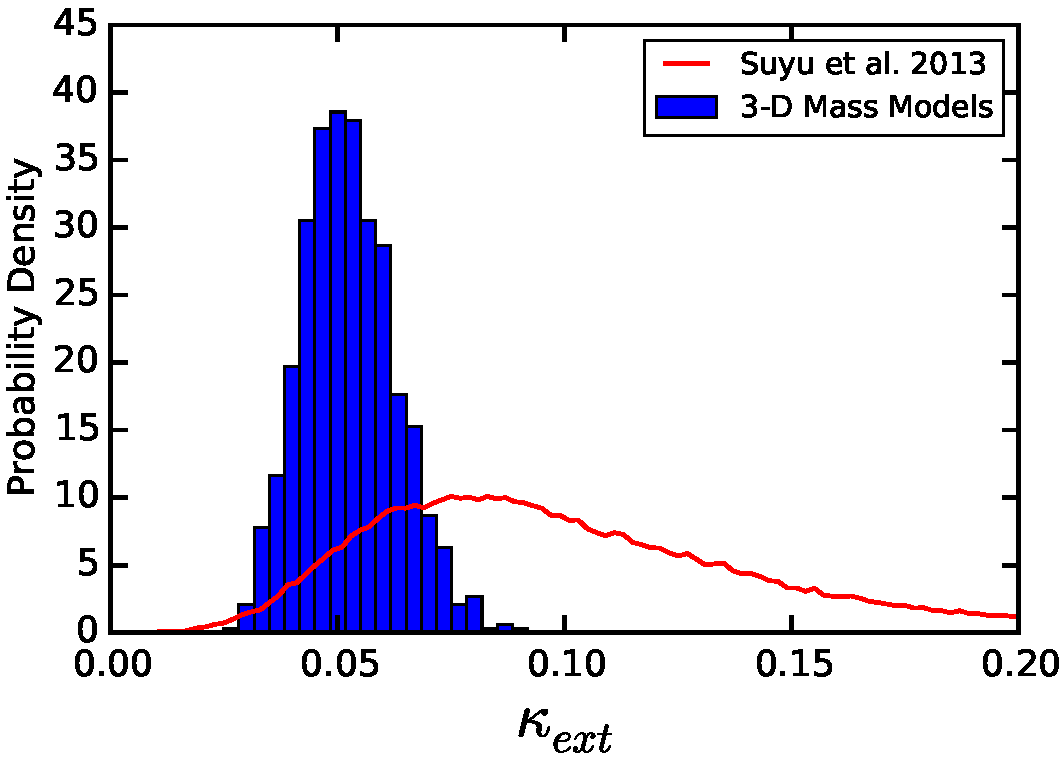
\includegraphics[width=0.7\columnwidth]{figures/suyu_kappa/suyu_kappa}
\caption{\label{fig:suyu} Probability distribution for the external convergence in the RXJ1131 field. The blue histogram shows effective convergence computed directly from our 3-D mass models, accounting for measurement uncertainties and scatter in the relations used to assign masses to galaxies. The red curve shows the external convergence distribution derived from the Millennium simulation by \citet{Suyu13}. The peaks of the distributions match well. Because we build mass models for the specific, observed field, we obtain a narrower distribution that effectively translates into a stronger prior on the Hubble constant.%
}
\end{center}
\end{figure}

We have argued that external convergence does not properly capture all LOS effects.  Nevertheless, it is a useful quantity to compare to previous works. \citet{Suyu13} used the Millennium simulation along with galaxy number counts around RXJ1131 to estimate their prior probability distribution for the external convergence used to constrain the Hubble constant; their distribution is shown in red in Figure \ref{fig:suyu}. We compute the effective convergence (as defined in M14 and references therein) directly from our mass model for RXJ1131.  We consider many realizations that account for observational uncertainties and scatter in the relations used to assign masses to galaxies \citep[see][]{Wong11}.  This yields a distribution of ``direct'' convergence calculations that is shown by the blue histogram in Figure \ref{fig:suyu}. We find that the peaks of the distributions match closely. However, our 3-D Lens models produce a tighter distribution of convergence values. This is likely because we build mass models based on the observed beam for each individual lens rather than using statistical results from N-body simulations. The narrower distribution of external convergences translates into a stronger prior on measuring the Hubble constant.


%%%%%%%%%%%%%%%%%%%%%%%%%%%%%%%%%%%%%%%%
\section{Which Image Configurations Produce the Strongest Constraints on Cosmology?}
\label{sec:ImageConfigs}
%%%%%%%%%%%%%%%%%%%%%%%%%%%%%%%%%%%%%%%%

Finally, we explore how changing the lens properties affects our results.

\begin{figure}[t]
\begin{center}
%crk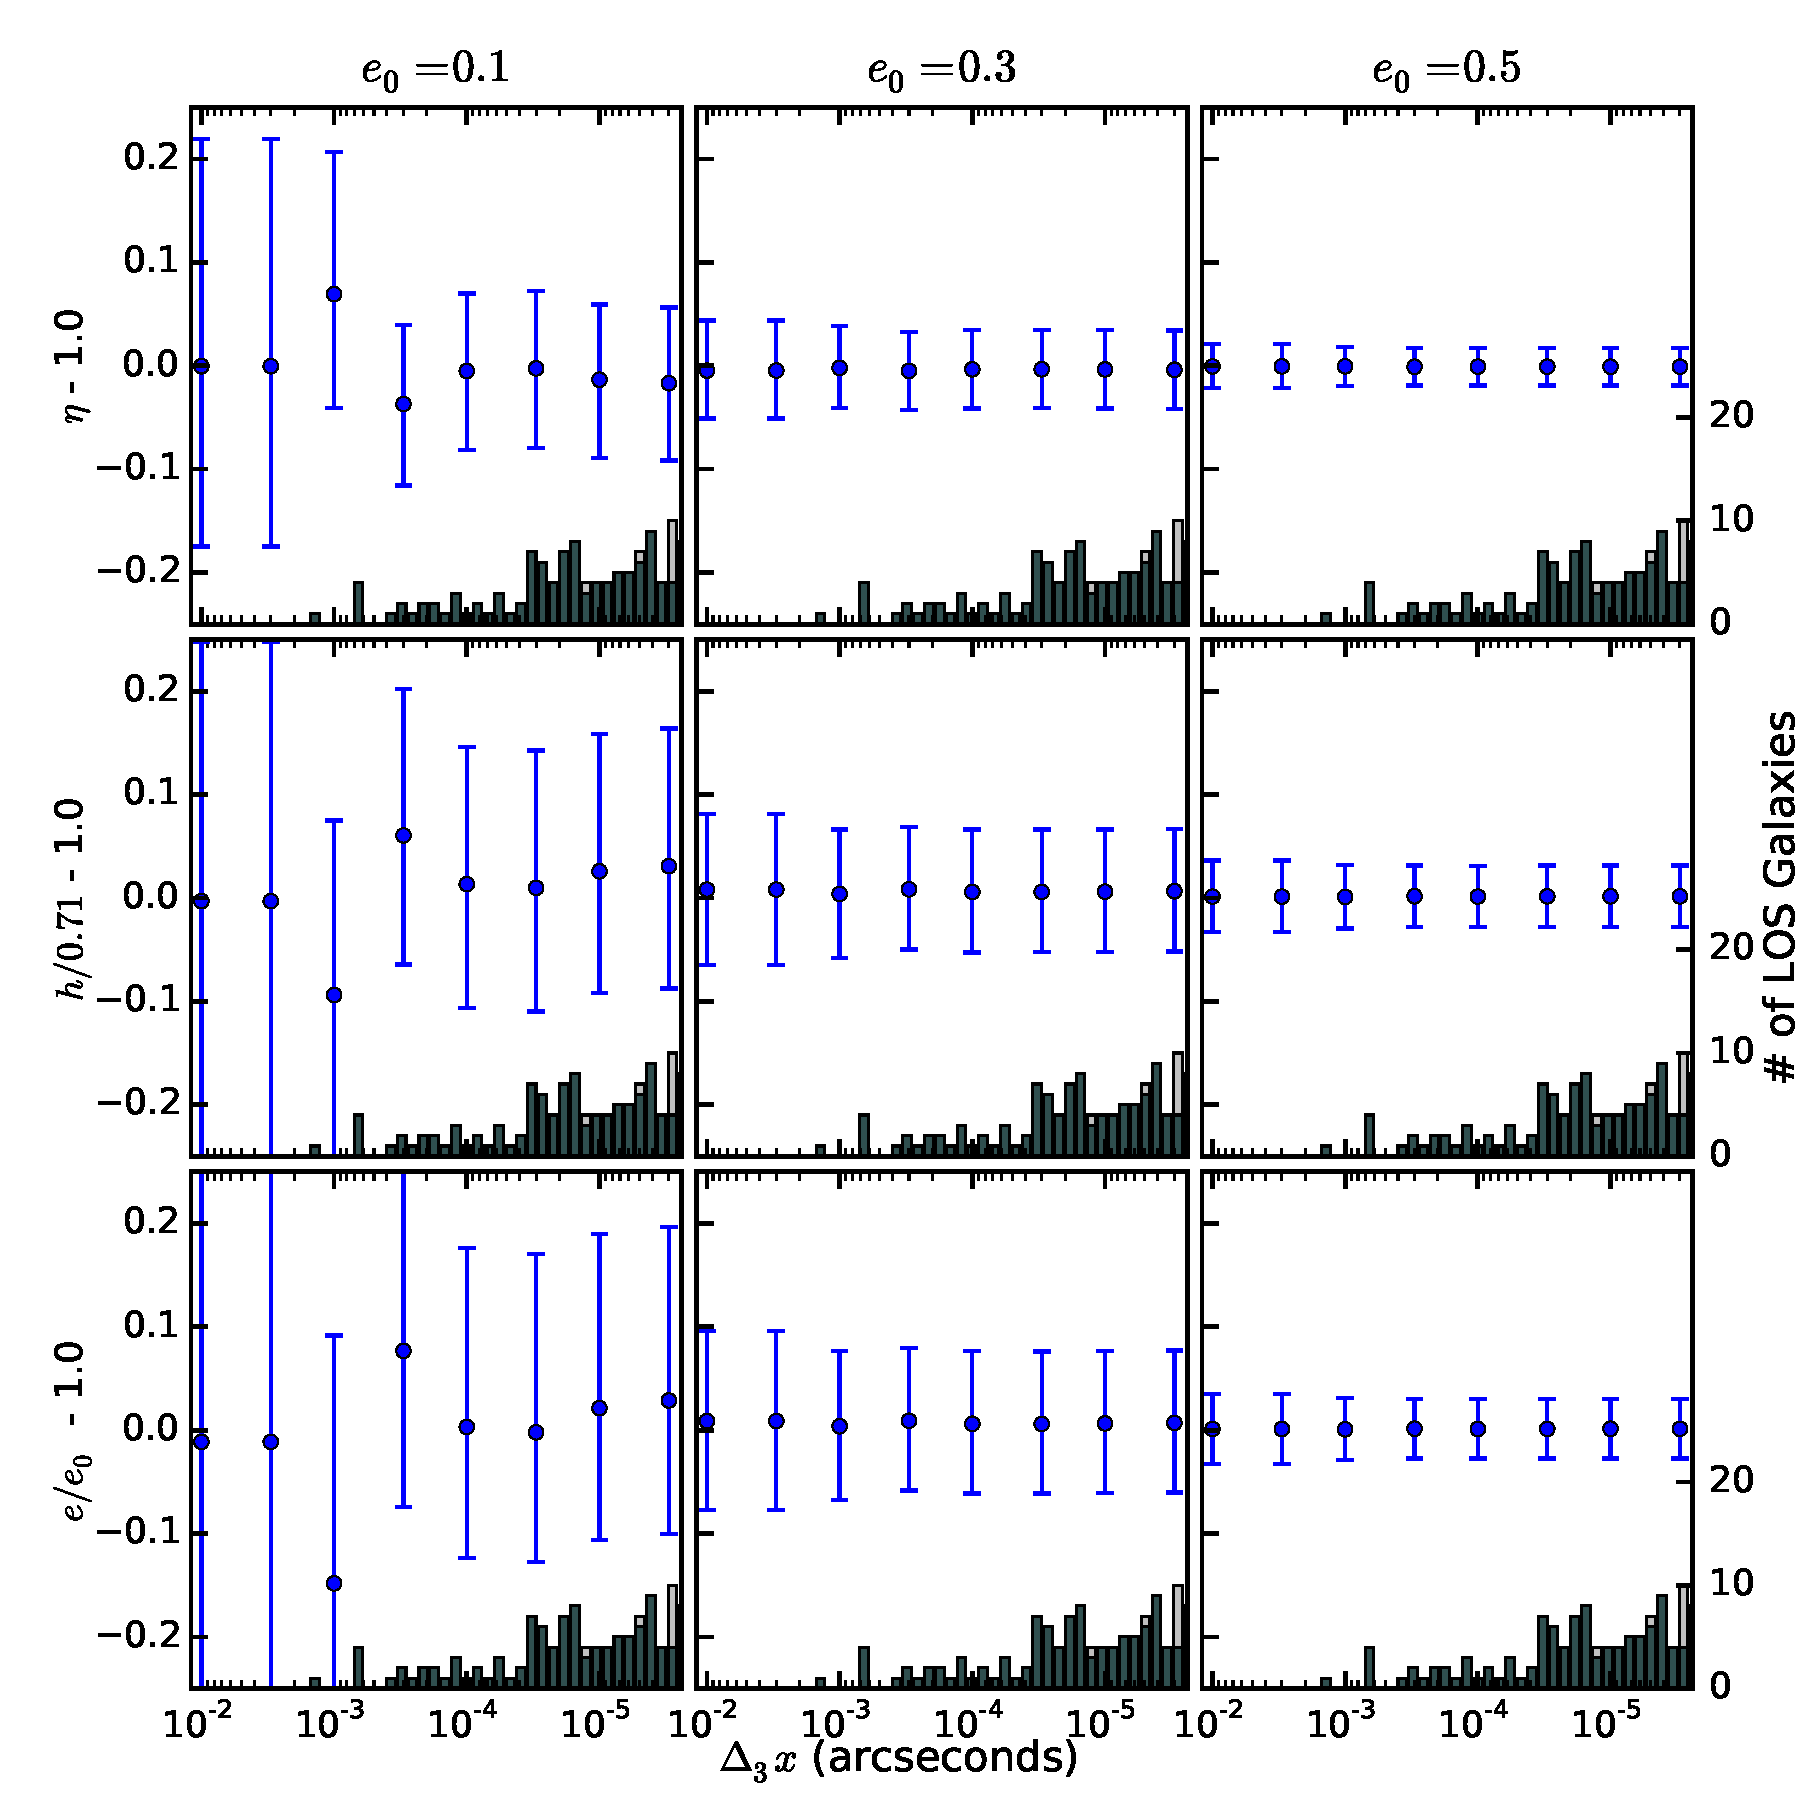
\includegraphics[width=1\columnwidth]{figures/ecompare/ecompare}
\caption{\label{fig:ecompare} Recovered model parameters for main lens galaxies with different ellipticities, using the RXJ1131 field with 3-D Lens models. The columns correspond to $e = 0.1,0.3,0.5$ from left to right. Systems with larger $e$ have less scatter in the power law index, $\eta$, and the Hubble constant, $h$. More asymmetric image configurations span a wider range of radii and provide strong constraints on the ellipticity, breaking the lens profile degeneracy and producing tighter constraints on the Hubble constant.%
}
\end{center}
\end{figure}

One important parameter that influences lens configurations is the ellipticity of the main lens galaxy.  Figure \ref{fig:ecompare} compares models results for different values of $e$.  As the ellipticity increases, the scatter in the recovered Hubble constant decreases. The configurations of very asymmetric lenses can only be produced for a smaller range of lens models, leading to stronger constraints on both the ellipticity and the power law index.  Since those parameters are correlated with the Hubble constant through the lens profile degeneracy, reducing the range of $e$ and $\eta$ leads to a narrower range for $h$ as well.

\begin{figure}[t]
\begin{center}
%crk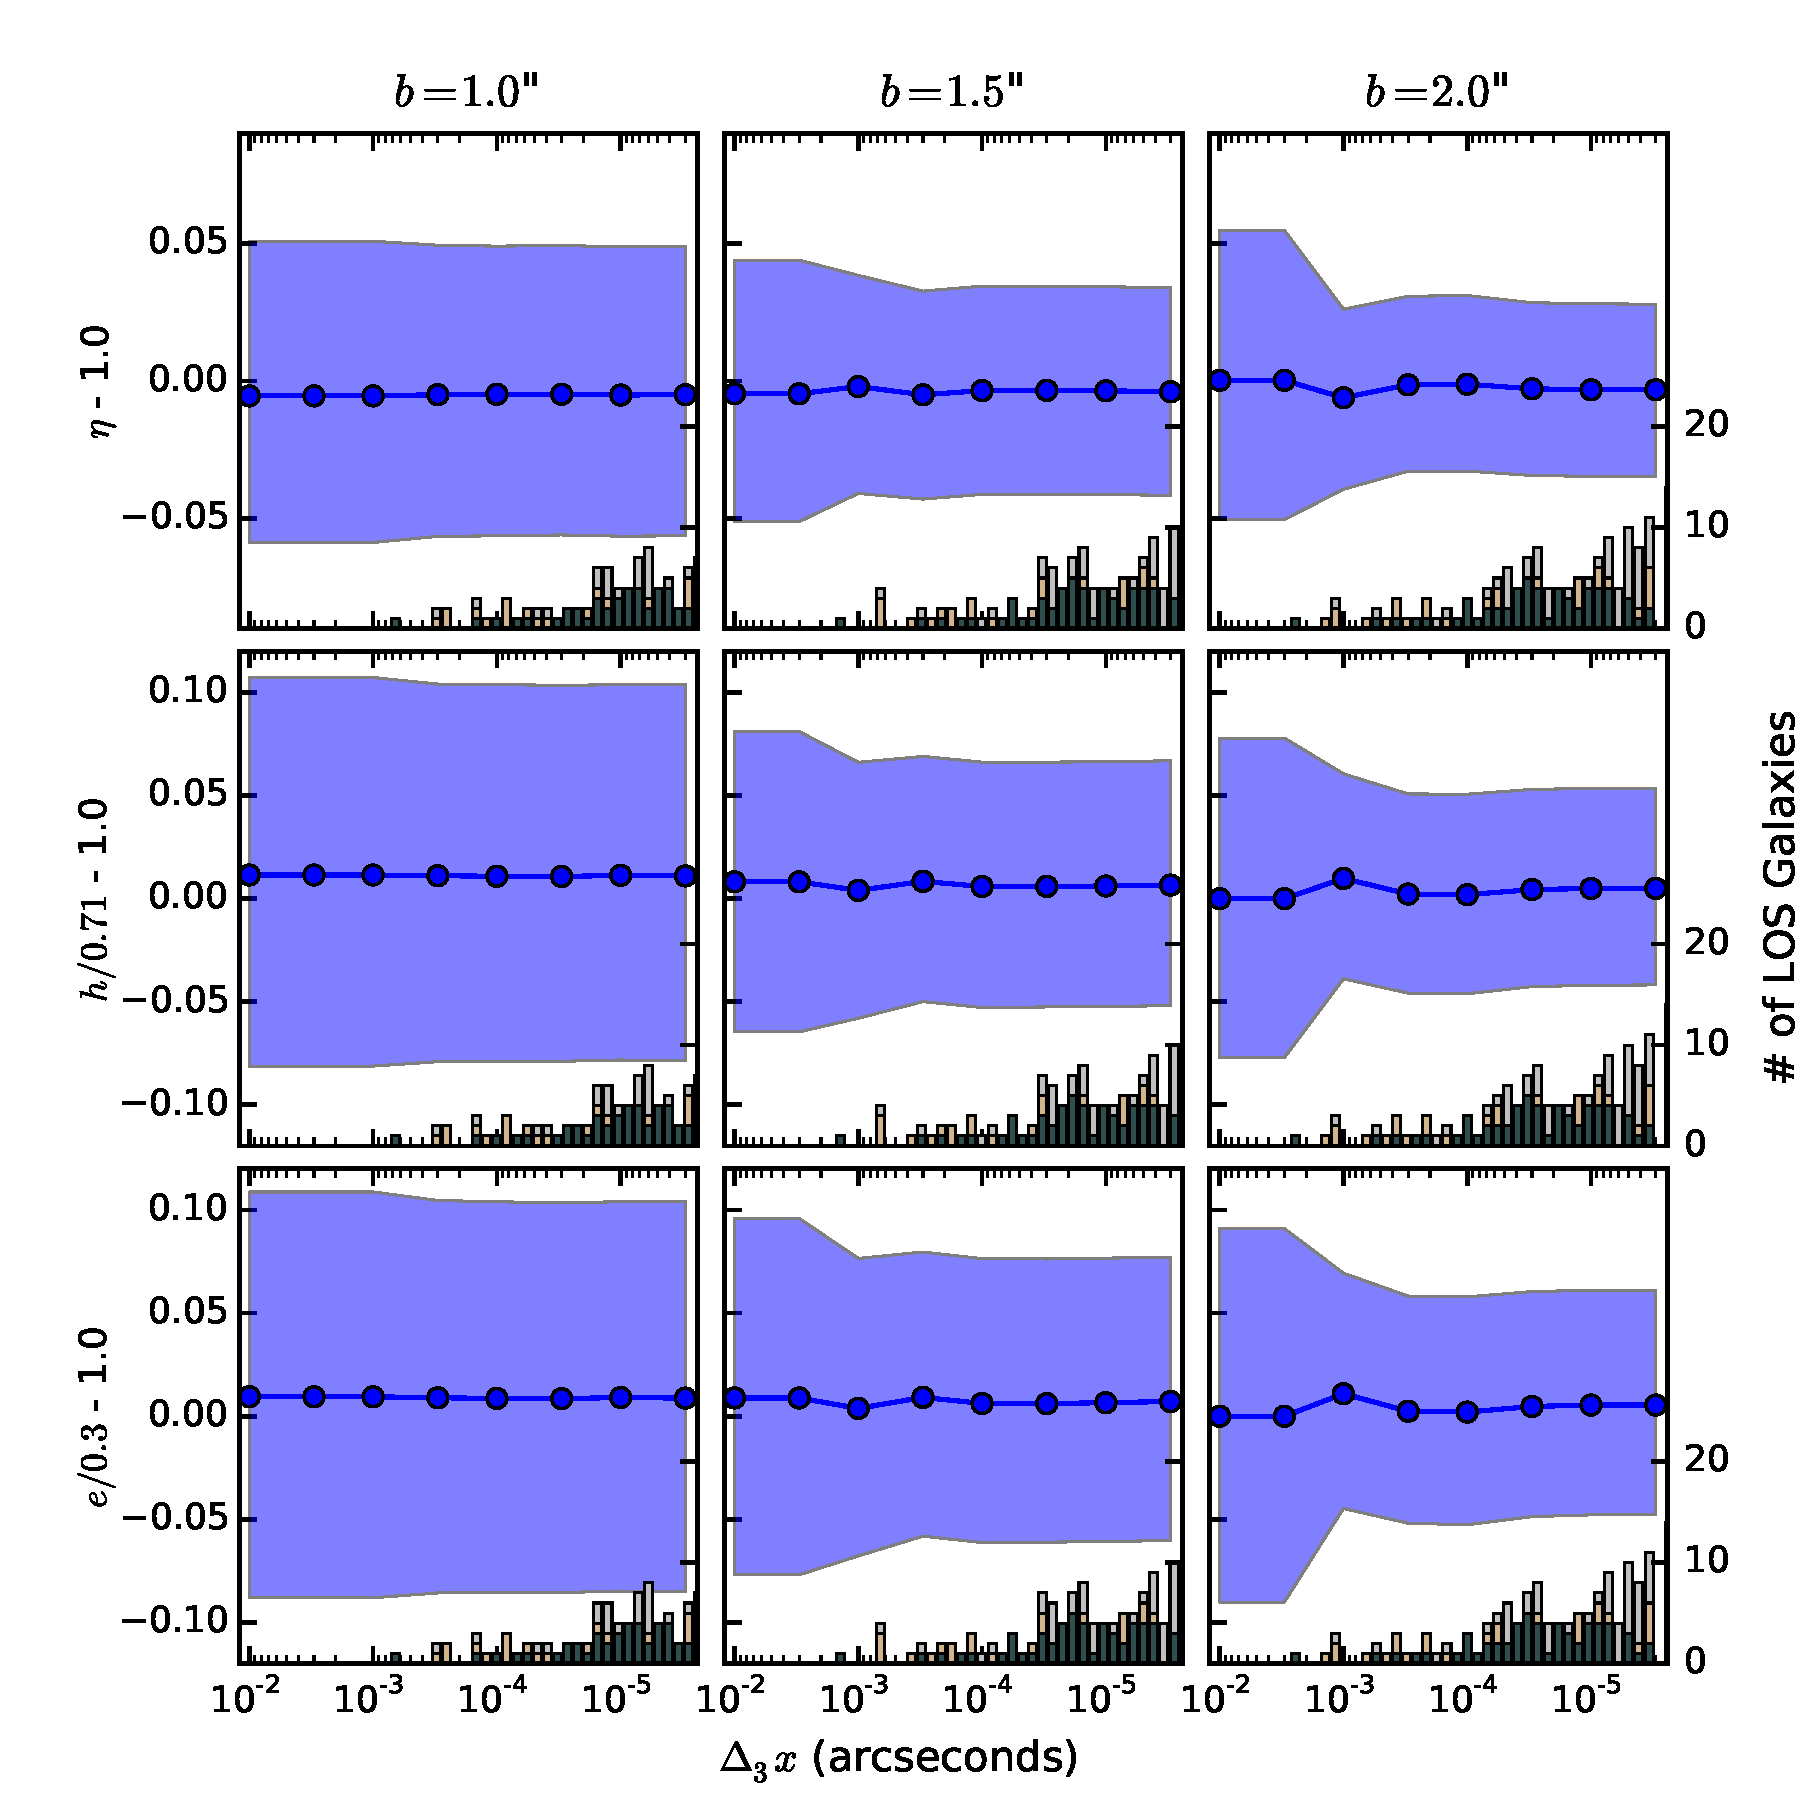
\includegraphics[width=1\columnwidth]{figures/recompare/recompare}
\caption{\label{fig:recompare} Similar to Figure \ref{fig:ecompare} but for different values of the Einstein radius parameter: $b = 1.0,1.5,2.0$ from left to right. Systems with a smaller Einstein radius have more scatter in the Hubble constant. Constraints on the ellipticity are somewhat stronger for lenses with larger Einstein radii, especially once the few strongest perturbers are included in models. This implies that lenses with a large Einstein radius should produce the strongest constraints on the Hubble constant.%
}
\end{center}
\end{figure}

A second key parameter of the main lens galaxy is the Einstein radius. Figure \ref{fig:recompare} shows model results for different values of the Einstein radius parameter $b$.  As the Einstein radius increases, the constraints on the Hubble constant get stronger. Lenses with large Einstein radii produce stronger constraints on the ellipticity limiting the lens profile degeneracy, yielding a tighter distribution on the Hubble constant.
  
LSST will find an immense number of new strong lens systems. There are various strategies about how to use this upcoming dataset for cosmology. One possibility is to use all of the lenses to beat down  uncertainties using statistics. However, if we are entering the systematics-limited regime, this approach will succeed only if one can account for systematic uncertainties (e.g., with our 3-D Lens models). An alternative strategy is to use the large number of lenses discovered by LSST to search for a few rare, ``golden'' lenses that have small systematic uncertainties. One possible criterion for a ``golden'' lens could be to have a have weaker contribution from the environment/LOS (see Figs.\ \ref{fig:allfields} and \ref{fig:d3xsums}). Based on our analysis above, to minimize environment/LOS effects, we should search for lenses with a large Einstein radius and high ellipticity. These large, asymmetric lenses will be less sensitive to the lens profile degeneracy. While suggestive, these results merit further investigation to get the most out of future surveys like LSST.
  
\begin{figure}[t]
\begin{center}
%crk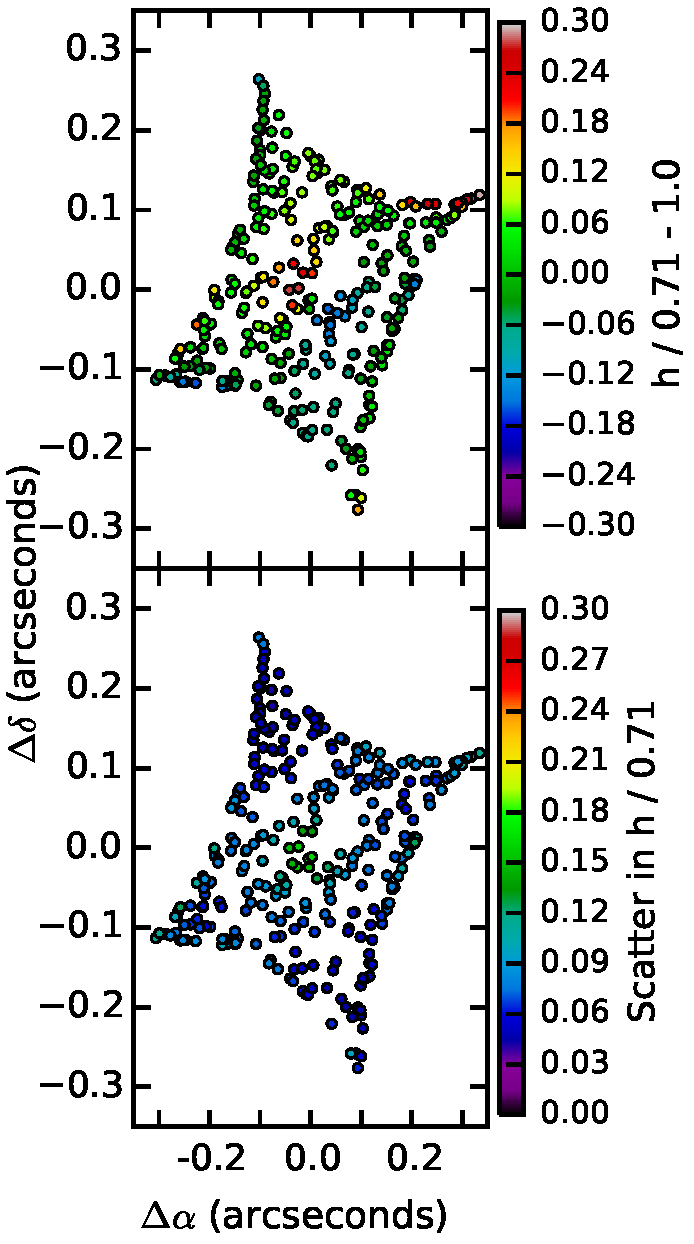
\includegraphics[width=1\columnwidth]{figures/h_src_pos/h_src_pos}
\caption{\label{fig:srcpos}
Median value (top) and scatter (bottom) for the recovered Hubble constant as a function of source position for the 3-D lens models. The models have little bias and small scatter near caustics, but show an increased scatter/bias near the center. These central source positions correspond to more symmetric image configurations which produce weaker constraints on the ellipticity and are therefore more susceptible to the lens profile degeneracy.%
}
\end{center}
\end{figure}

Now that we have established some of the qualitative trends about 3-D lensing, we turn to a more direct comparison with the real RXJ1131 system. \citet{Suyu13} find the best fit parameters of RXJ1131 to be $b = 1.64$'', $\eta = 1.05$, $e = 0.237$, and $\theta_e = 115.8^{\circ}$. We generate mock data for this configuration and then perform a modeling analysis as above. Here we treat all perturbers using the 3-D tidal approximation.

Figure \ref{fig:srcpos} shows the median and scatter in the best fit Hubble constant as a function of source position. The models do well when the source is near a caustic. However, near the center of the caustic, both sets of models have larger scatter in the recovered values for the Hubble constant. These source positions correspond to more symmetric image configurations, with the exact center producing an Einstein ring. Symmetric image configurations produce weaker constraints on the ellipticity than asymmetric image configurations and are therefore more susceptible to lens profile degeneracy as discussed above.


%%%%%%%%%%%%%%%%%%%%%%%%%%%%%%%%%%%%%%%%
\section{Conclusions}
%%%%%%%%%%%%%%%%%%%%%%%%%%%%%%%%%%%%%%%%

As lensing data improve, it becomes more important to take into account systematic effects like the perturbations due to galaxies in the environment and along the LOS. Our results show that if we want to do ``precision lensing,'' the environment/LOS cannot be ignored.

We find that perturbers in the foreground of the lens affect the lens potential more than those in the background for two different reasons. The first is that background perturbers are downweighted; a background perturber must be closer in projection to have the same effect as a foreground perturber. The second is that while background perturbers can be mimicked by a shear in the lens plane, foreground perturbers can not. Foreground perturbers create non-linear effects that cannot be fit with a simple external shear.

When accounting for the environment, our 3-D Lens models produce results that do not have significant bias and have less scatter than models that fit with a Lens+Shear. The Lens+Shear models also overpredict the Hubble constant and the Einstein radius of the main lens galaxy; these quantities need to be corrected using some other constraint on the external convergence. Our LOS framework does not produce the biases seen here because we explicitly include the convergence in the mass models.

For either methodology of fitting an external shear or using our LOS framework, we still must choose which galaxies are treated exactly and which are treated in the tidal approximation. We find that we can reproduce the true lens parameters with no bias with scatter less than the observational uncertainties if we use a cutoff in $\Delta_3 x$ of $10^{-4}$ arcseconds, a factor of 30 smaller than the assumed uncertainties on the observed positions. This cut typically requires 10-15 galaxies to be treated exactly, making the calculation $\sim 400$ times more efficient than the full multi-plane lens equation.

We find that the importance of environment/LOS effects varies significantly from field to field. Therefore, we argue that each field needs to be modeled individually. We find that lens galaxies that are in groups tend to have a stronger contribution from the ENV/LOS than those that are not in groups. Accounting for the uncertainties in building the 3-D mass models, we find that the distribution of external convergence is narrower for our 3-D Lens models than from ray tracing through N-body simulations. This translates to a stronger prior on measuring the Hubble constant.

We show that the all models, including both the Lens+Shear and 3-D Lens models, are subject to the lens profile degeneracy in agreement with \citet{Xu15,Schneider13}. We find that highly asymmetric lenses are less sensitive to this degeneracy.

One possible approach to using gravitational lensing for precision cosmology is to search for one or a few ``golden lenses'' to use to measure cosmological parameters. One consideration when choosing these lenses needs to be the environment. We find that there is significant diversity in lens LOS/environments, with both the number and strengths of the perturbing galaxies vary from field to field.  We also examine which lens properties affect the sensitivity to the environment/LOS. We find that asymmetric image configurations, e.g. those produced by a highly elliptical main lens galaxies, are less sensitive to the lens profile degeneracy leading to improved constraints on the Hubble constant.

Throughout this work we have assumed that our 3-D models perfectly describe the environment/LOS, but there is also uncertainty in generating the environment mass models that is only briefly addressed here. This source of uncertainty will be explored in a forthcoming paper (Wong et al., in prep.).

\acknowledgements
We thank Phil Marshall, Sherry Suyu, Chris Fassnacht, and Stefan Hilbert for enlightening discussions about 3-D lensing. CVM acknowledges support from NSF grant AST-1313484. CRK acknowledges funding from NSF grant AST-1211385. AIZ acknowledges funding from NSF grant AST-1211874 and NASA grant ADP-10AE88G. She also thanks the John Simon Guggenheim Foundation and the Center for Cosmology and Particle Physics at NYU for their support. KCW is supported by XXXXXX.


\bibliographystyle{apj}
\bibliography{sims.bib}

\end{document}